\documentclass[a4paper,12pt]{book}
\usepackage[utf8]{inputenc}
\usepackage{graphicx}
\usepackage{amsmath}
\usepackage{amssymb}
\usepackage{wrapfig}
\usepackage{hyperref}
\usepackage{multicol}
\usepackage{dirtytalk}
\usepackage{algpseudocode}
\usepackage{xcolor}

\hypersetup{
	colorlinks=true,
	linkcolor=blue,
	citecolor=green,
	filecolor=magenta,
	urlcolor=cyan
}

\begin{document}

\author{TeXstudio Team}
\title{Simple Book Example}
\date{January 2013}

\frontmatter
\maketitle
\tableofcontents

\mainmatter
\chapter{Introduzione}
\section{Cos'è un immagine?}
\subsection{Definizioni}
Un'immagine $f(x,y)$ è una rappresentazione su un piano 2D di:
\begin{itemize}
	\item una scena o un fenomeno fisico misurabile;
	\item un modello definito analiticamente.
\end{itemize}
A seconda di come si ottiene l'immagine si parla di:
\begin{description}
	\item[Immagini visibili] quelle che possono essere viste dall'occhio umano o sono catturate da un sistema ottico;
	\item[Immagini non direttamente visibili] generate a partire da una distribuzione di grandezze fisiche come ad esempio una mappa di temperature;
	\item[Immagini definite da modelli analitici] ottenute a partire da funzioni continue o discrete, come la sintesi di modelli 3D.
\end{description}
Le immagini possono essere analogiche, caratterizzate da funzioni continue $f(x,y)$ che definiscono il colore e l'intensità luminosa oppure \textbf{digitali}, nelle quali la funzione di prima viene approssimata due volte:
\begin{itemize}
	\item campionando: il piano $XY$ viene diviso con una griglia e consideriamo un solo valore di colore per ogni cella della griglia (la chiameremo pixel)
	\item quantizzando: dovendo immagazzinare l'informazione del pixel in un calcolatore non abbiamo a disposizione infinita precisione, dovremo perciò troncare il valore
\end{itemize}
\subsection{Ottenere un'immagine}
Dal punto di vista tecnico per ottenere un'immagine campionata e quantizzata con una fotocamera si fa arrivare con il sistema ottico la luce al sensore, il sensore è diviso in celle che permettono di ottenere ciascuna un pixel (campionamento o sampling), ogni cella traduce l'intensità luminosa che la colpisce in un segnale elettrico che viene tradotto in un valore tipicamente intero tra 0 e 255 (quantizzazione). Per ottenere L'immagine a colori si sovrappone al sensore una griglia colorata che permetta a ogni cella del sensore di assorbire solo la luce di un certo colore (RGB)
\subsection{Quantizzazione}
il valore di ogni pixel deve essere espresso attraverso un certo numero finito di bit, più bit usiamo più saremo in grado di definire colori differenti, il numero di bit è quindi detto \textbf{color depth} o \textbf{profondità di colore} e si indica con l'acronimo \textbf{bpp} cioè bit per pixel. Se un immagine è in bianco e nero significa che per ogni pixel salviamo un solo bit, l'immagine è detta \textbf{binarizzata}

Normalmente usiamo 8 bit per esprimere un valore, da questo segue che un'immagine in scala di grigi avrà 256 livelli di grigio. Per le immagini a colori dividiamo il valore del pixel nelle componenti RGB detti anche \textbf{canali}, destiniamo a ogni canale 8 bit ottenendo 16 milioni di colori circa.

\section{Operazioni con le immagini}
Possiamo definire delle operazioni sulle immagini che prendano in input una o due immagini e restituiscano uno scalare, un vettore o un'altra immagine
\subsection{Operazioni pixel a pixel}
\subsubsection{Operazioni logiche}
Si applicano a due immagini binarizzate aventi la stessa dimensione e si ottiene una terza immagine in cui ogni pixel è il risultato dell'operazione logica sui pixel corrispondenti nelle immagini iniziali.
\subsubsection{Operazioni aritmetiche}
Possiamo applicarle a due immagini di qualsiasi tipo purché con la stessa dimensione. Il risultato è un'immagine in cui ogni pixel è ottenuto applicando una certa funzione aritmetica ai pixel di partenza corrispondenti. Quando si lavora con queste operazioni si deve tenere conto della possibilità di sforare il range di rappresentazione dei pixel, il risultato dovrà essere quindi opportunamente clippato o scalato.
\subsubsection{Trasformazioni affini}
Queste operazioni permettono di traslare, scalare, ruotare e fare shear di un'immagine, facendo in modo che le linee dritte rimangano tali. Queste operazioni si implementano con \textbf{matrici} di \textbf{trasformazione} $T$.
\begin{equation}
	\begin{bmatrix}
		x'\\
		y'\\
		1
	\end{bmatrix}
	= 
	\begin{bmatrix}
		c_{11} & c_{12} & c_{13} \\
		c_{21} & c_{22} & c_{23} \\
		0 & 0 & 1 \\
	\end{bmatrix}
	\times
	\begin{bmatrix}
		x\\
		y\\
		1
	\end{bmatrix}
	= T \times
	\begin{bmatrix}
		x'\\
		y'\\
		1
	\end{bmatrix}
\end{equation}
\subsection{Operazioni su più pixel}
Le operazioni che coinvolgono più pixel di una certa immagine sono tipicamente implementate mediante \textbf{filtri} queste operazioni sono importantissime e ne parleremo più approfonditamente in seguito (\ref{asd}).

\section{Dimensione dell'immagine}\label{sec:image_dimension}
Quando si parla di dimensione si intende il numero di pixel che costituiscono l'immagine, dato che le immagini sono tipicamente rettangolari e i pixel sono organizzati in una griglia la dimensione dell'immagine si ottiene moltiplicando la base per l'altezza.

Una volta ottenuta la dimensione è facile calcolare lo \textbf{spazio occupato} dall'immagine, se usiamo 8 bit per canale e abbiamo 3 canali basta moltiplicare per 3 la dimensione dell'immagine per avere la sua occcupazione in byte. Si vede che questa, anche per immagini non grandissime è molto elevata, nel tempo quindi si sono sviluppati efficientissimi algoritmi di compressione delle immagini; ne parleremo più avanti (\ref{asd}).
\subsection{Risoluzione}
La risoluzione ci da un'idea di quanto possa essere gradevole guardare un'immagine senza vedere la grana dei pixel. Per questa ragione è una funzione della dimensione e dell'area fisica su cui l'immagine viene stampata o proiettata. In particolare la risoluzione si ccalcola in \textbf{punti per pollice} (dpi) e vale la seguente relazione:
\begin{equation}
	dimensione = area \cdot risoluzione
\end{equation}

\section{Campionamento}
Quando acquisiamo un'immagine reale stiamo discretizzando un fenomeno fisico, dalla teoria dell'informazione conosciamo il \textbf{teorema di Nyquist-Shannon} che afferma che se vogliamo campionare correttamente dobbiamo usare una frequenza di campionamento almeno pari al doppio della frequenza massima presente nel segnale che vogliamo acquisire.

Nelle immagini le alte frequenze corrispondo a bordi di colori molto diversi ravvicinati fra loro, mentre la frequenza di campionamento è data da quanto è fitta la griglia di celle del nostro sensore. Quando acquisiamo un immagine non possiamo fare come nell'audio e usare dei filtri passa basso per eliminare le frequenze troppo alte, perché questo equivarrebbe a sfocare l'immagine. Possono pertanto presentarsi degli artefatti dovuti all'errato campionamento di determinati pattern; questi sono detti \textbf{Moiré}.
\chapter{Il Colore}
\section{Descrizione fisica}
\subsection{Definizioni}
Il colore è la traduzione da parte del nostro cervello di un fenomeno fisico. Possiamo descrivere questo fenomeno come uno spettro che assegna a ogni lunghezza (o frequenza) d'onda visibile la sua energia. Sullo spettro definiamo:
\begin{description}
	\item[Lunghezza d'onda dominante] la lunghezza d'onda della componente più energetica, è detta anche \textbf{hue}
	\item[Saturazione] il rapporto tra l'energia della hue e il valor medio dello spettro (luce bianca)
	\item[Radianza] l'energia emessa da una certa sergente (è l'integrale dello spettro)
	\item[Luminanza] energia percepita da un osservatore
	\item[Brightness] intensità della componente acromatica
	\item[Cromaticity] o \textbf{chroma} hue + saturazione
\end{description}

\section{Modelli di colore}\label{sec:color_model}
Per descrivere un colore si possono usare vari modelli che differiscono nel modo di rappresentare l'informazione, ma sono tutti equivalenti e hanno la stessa capacità espressiva Questi modelli definiscono dei volumi di colore in cui ciasun punto rappresenta un colore diverso, sono per questo detti \textbf{spazi colore}.
\subsection{Cubo RGB}
In questo modello si definisce un cubo di lato 1 avente un vertice nell'origine degli assi. Ogni asse rappresenta una componente e ogni punto all'interno del cubo sarà un colore avente un ben preciso rapporto tra le componenti. Questo modello è molto semplice e adatto a un calcolatore, ma è difficile da usare per gli umani, sono state quindi proposte alternative.
\subsection{Modelli HS*}
Questa famiglia di modelli si basano sul modo umano di rappresentare il colore e descrivono 
\begin{itemize}
	\item \textbf{Hue}: la tinta del colore
	\item \textbf{Saturazione}: quanto il colore è puro
	\item \textbf{Luminosità}: quanto ci appare brillante
\end{itemize}
Tutti i modelli HS* sono derivati applicando delle trasformazioni al cubo RGB, in particolare in tutti i modelli si ruota il cubo in modo che la diagonale che congiunge il bianco al nero sia verticale.

\begin{wrapfigure}{r}{.5\linewidth}
	\hspace{.09\linewidth}
	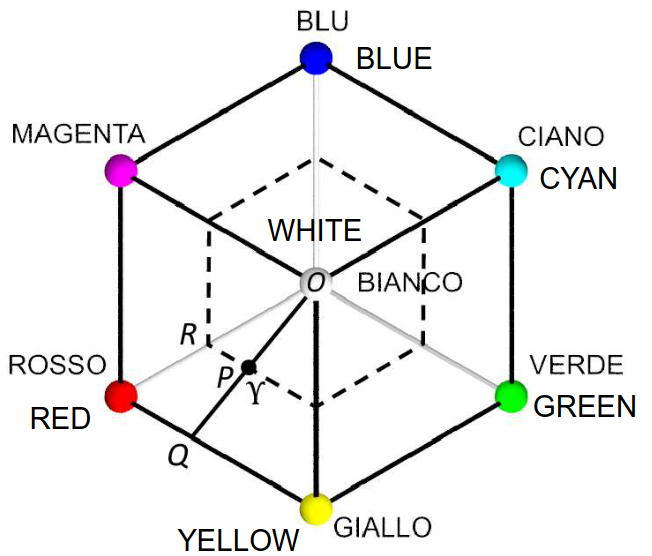
\includegraphics[width=.9\linewidth]{Picture/Cromaticity_Plane}
\end{wrapfigure}
Il piano che si ottiene guardando dall'alto i cubo ruotato è detto \textbf{chromaticity plane}. Su questo si definisce la \textbf{chroma} e la \textbf{hue} del colore $\Upsilon$
\begin{align}
	chroma(\Upsilon) &= \frac{OP}{OQ}\\
	hue(\Upsilon) &= \frac{RP}{6OR}
\end{align}

Cioè la chroma è il rapporto tra la distanza del colore dal bianco e la distanza dal bianco della tinta pura; mentre la hue è il rapporto tra la distanza dal rosso (in senso orario) e il perimetro dell'esagono.
\subsection{Spazio HSV}
In questo spazio il piano della cromaticità viene alzato fino al bianco, si rende questo esagono un cerchio e la base si trasforma in un cerchio nero, ottenendo alla fine un cilindro. Hue e croma sono definite come prima, si aggiunge il $value(\Upsilon)$ che rappresenta l'altezza sul cilindro. Si definisce poi la saturazione come:\\
\begin{minipage}{.8\linewidth}
	\vspace{-.5cm}
	\begin{equation}
		saturation(\Upsilon) = 
		\begin{cases}
			0 & if\ value(\Upsilon) = 0 \\
			\frac{chroma(\Upsilon)}{value(\Upsilon)} & otherwise
		\end{cases}
	\end{equation}
\end{minipage}
\hspace{.05\linewidth}
\begin{minipage}{.15\linewidth}
	\centering
	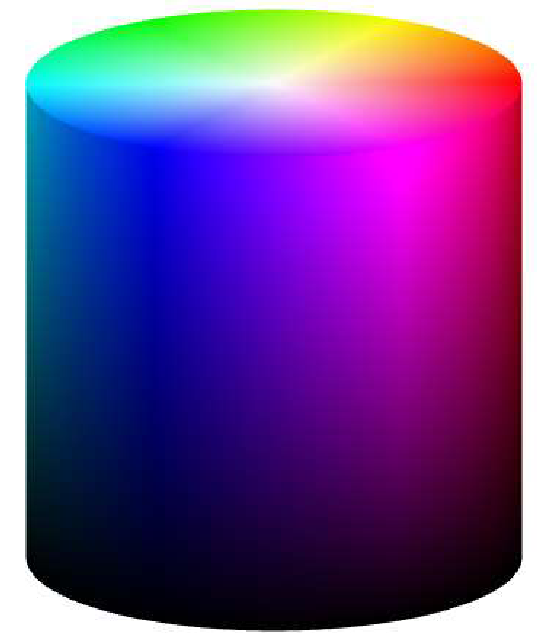
\includegraphics[width=.9\linewidth]{Picture/HSV_Space}
\end{minipage}

\subsection{Spazio HSL}
Anche in questo spazio colore si ottiene un cilindro ma il piano della cromaticità rimane al centro, mentre la faccia superiore è completamente bianca e quella inferiore completamente nera. In questo caso l'altezza sul cilindro si chiama $lightness(\Upsilon)$ (abbreviata nella formula sotto con $light$). La saturazione invece è:\\
\begin{minipage}{.8\linewidth}
	\vspace{-.5cm}
	\begin{equation}
		saturation(\Upsilon) = 
		\begin{cases}
			0 & light(\Upsilon) = 0\ \text{or}\ 1 \\
			\frac{chroma(\Upsilon)}{1 - |2\cdot light(\Upsilon) -1} & otherwise
		\end{cases}
	\end{equation}
\end{minipage}
\hspace{.05\linewidth}
\begin{minipage}{.15\linewidth}
	\centering
	\includegraphics[width=.9\linewidth, height=2cm]{Picture/HSl_Space}
\end{minipage}
\subsection{Spazio HSI}
È un modello che cerca il migliore compromesso tra comodità di rappresentazione ed efficienza sul calcolatore. Si parte sempre dal cubo ruotato, per poi normalizzarlo in modo che la diagonale sia lunga 1. In questo modello definiamo l'intensità $I$ come la somma delle componenti colorate diviso tre e la saturazione come 1 meno la componente più piccola, tutto diviso l'intensità. Con queste definizioni il modello rimane comodo per un utilizzatore e la conversione nelle componenti RGB risulta molto efficiente.

\section{Trasformazioni di colore}
\subsection{Trasformazioni in Pseudocolore}
Un immagine in scala di grigi con una profondità colore di 8 bit permette di avere 256 livelli di grigio differenti, nelle immagini mediche la profondità colore è ancora maggiore. L'occhio umano però non è sensibile a così tanti livelli di grigio, per migliorare la percezione si può trasformare una immagine monocromatica in una a falsi colori. 
\subsubsection{Intensity slicing}
\begin{wrapfigure}{r}{.4\linewidth}
	\centering
	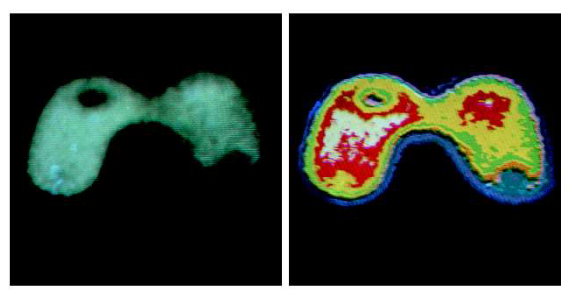
\includegraphics[width=.9\linewidth]{Picture/Pseudocolor}
\end{wrapfigure}
È una particolare trasformazione in pseudocolori che consiste nell'associare a ogni range di valori in scala di grigi un colore. In questo modo ogni pixel è colorato in base al suo livello di intensità. Come si vede dall'esempio questo metodo permette di distinguere molto meglio le varie zone dell'immagine.
\subsection{Trasformazione in falsi colori}
In questo caso si parte da un immagine a colori e si mappano i vari colori su altri colori, a esempio per evidenziare particolari dettagli. Una trasformazione di questo tipo può essere espressa come matrice di trasformazione che prende come input il vettore che contiene le componenti di colore di ciascun pixel:
\begin{equation}
	\begin{bmatrix}
		R'\\
		G'\\
		B'
	\end{bmatrix}
	= 
	\begin{bmatrix}
		c_{11} & c_{12} & c_{13} \\
		c_{21} & c_{22} & c_{23} \\
		c_{31} & c_{32} & c_{33} 
	\end{bmatrix}
	\times
	\begin{bmatrix}
		R\\
		G\\
		B
	\end{bmatrix}
\end{equation}

\chapter{Image Processing}
In questo capitolo vediamo brevemente i principali tipi di processing di immagini e tipo per tipo quali sono gli obiettivi della manipolazione.

\section{Image enhancement}
Questo tipo di processing ha lo scopo di migliorare l'immagine in modo \textbf{soggettivo} e mirato alle elaborazioni future, è quindi un trattamento a monte prima di utilizzare l'immagine per ulteriori manipolazioni. Elaborazioni tipiche di enhancement sono la riduzione del rumore e miglioramento del contrasto. 

L'image enhancement può anche essere l'unico step di processing e in questo caso ha lo scopo di rendere più gradevole l'immagine a un osservatore umano.

L'aspetto che caratterizza questa elaborazione è quella di essere application-driven, nel senso che la manipolazione è pensata ad hoc per il passo successivo a cui andrà incontro l'immagine (che sia quello di essere osservata oppure di essere ulteriormente elaborata).

\section{Image restoration}
Questa elaborazione ha lo scopo di aumentare la qualità dell'immagine in modo \textbf{oggettivo}, andando ad esempio a recuperare delle informazioni perse o correggendo errori fatti durante il processo di acquisizione. 

Per operare questo recupero di informazioni è necessario avere una conoscenza del dominio specifico e della funzione di degradazione che ha comportato la perdita di informazioni.

\section{Compressione}
Come accennato nel paragrafo sulla dimensione delle immagini (\ref{sec:image_dimension}) queste possono arrivare a occupare notevole spazio in memoria, la compressione si pone allora l'obbiettivo di ridurre lo spazio occupato dalle immagini, sia per risparmiare memoria sia per ridurre i tempi di trasmissione. Distinguiamo tra due tipi di compressione:
\subsection{Compressione lossless}
In cui l'immagine decompressa è esattamente identica all'immagine originale. Con questo tipo non si riescono a raggiungere livelli di compressione molto elevati, ha comunque senso in particolari applicazioni in cui è importante mantenere tutti i dati (ambito medico a esempio).
\subsection{Compressione lossy}
L'immagine decompressa è diversa dall'immagine originale, tipicamente siamo interessati a ottenere dei difetti impercettibili per l'occhio umano. Tecniche di compressione lossy si possono basare su
\begin{itemize}
	\item \textbf{sublsampling}: ridurre il numero di pixel memorizzati, per fare questo bisogna fare attenzione a non introdurre artefatti come le moiré;
	\item \textbf{ridurre la quantizzazione}: per ogni pixel riduciamo la profondità colore.
\end{itemize}
Queste tecniche si possono anche mischiare e rendere adattative, ad esempio usando una grana fine e una buona profondità colore per i soggetti a fuoco e riducendo la qualità per le parti non in evidenza.

\section{Segmentation}
Consiste nel partizionare un'immagine estraendo quelle parti alle quali siamo interessati. Anche questa elaborazione può essere fatta a monte di altre che ad esempio tentano di classificare le parti segmentate o cercano difetti nei componenti prodotti a cui è stata scattata una foto.

Dopo la segmentazione quindi è importante riuscire a rappresentare le parti segmentate e associare ad esse delle caratteristiche alle quali siamo interessati, ad esempio l'area di queste parti, il perimetro, la presenza di difetti, curvature ecc...
\chapter{Enhancement nel dominio spaziale}
In questo capitolo vediamo le principali tecniche di enhancement nel dominio dello spazio,ovvero modificando il valore dei pixel attraverso funzioni che prendono in input uno o più pixel dell'immagine che intendiamo trasformare.

Dividiamo il tipo di funzione che applichiamo all'immagine a seconda degli argomenti che prende in input:
\begin{description}
	\item[Trasformazioni puntuali] che operano pixel a pixel e sostanzialmente mappano i livelli di intensità in altri livelli;
	\item[Trasformazioni locali] prendono in input un pixel e i suoi vicine, sono quelle in assoluto più usate e sono chiamate \textbf{filtri};
	\item[Trasformazioni globali] prendono come argomento l'intera immagine, tipicamente non ci permettono di ottenere una nuova immagine, ma servono a estrarre informazioni globali sull'immagine.
\end{description}

\section{Trasformazioni puntuali}
Anche se queste funzioni permettono semplicemente di rimappare il livello di intensità pixel a pixel sono molto utili per ottenere immagini più ricche di informazione e correggere eventuali errori dovuti all'acquisizione o allo strumento di visualizzazione dell'immagine.

Sono inoltre queste trasformazioni che ci permettono di ottenere immagini in pseudocolori o in falsi colori. Queste trasformazioni sono particolarmente utili in ambito medico e scientifico, dove è necessario evidenziare dettagli su immagini ottenute attraveso sensori che catturano fenomeni non osservabili otticamente.
\subsection{Look Up Table}
\begin{wrapfigure}{r}{.4\linewidth}
	\vspace{-.6cm}
	\centering
	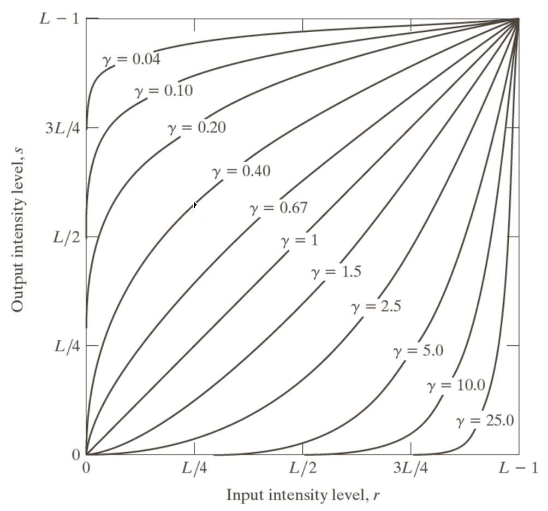
\includegraphics[width=.9\linewidth]{Picture/Gamma_Trasformation}
\end{wrapfigure}
I metodi che prevedono una funzione per rimappare i livelli di grigio solitamente si basano su Look Up Table (\textbf{LUT}) che specificano per ogni livello di grigio in ingresso il nuovo livello di grigio del pixel in uscita. Nell'immagine si può vedere una tipica trasformazione generata con una Power-Law, questa trasformazione serviva per correggere la gamma dei televisori a tubo catodico e prende quindi il nome di \textbf{gamma correction}.

\subsubsection{Tipologie di LUT}
Non c'è nessuna regola sul come costruire una LUT per rimappare i livelli di grigio, a seconda dell'obbiettivo che si vuole raggiungere si può costruire la LUT più adatta. Vediamo alcune tipologie particolarmente importanti:
\begin{itemize}
	\item \textbf{scala}: serve per ridurre il numero di livelli di grigio, opera una compressione lossy e può generare falsi bordi;
	\item \textbf{rampa}: serve per incrementare il contrasto in una particolare regione, ovviamente se si incrementa da una parte si riduce al di fuori della rampa;
	\item \textbf{binario}: permette di binarizzare l'immagine mettendo al massimo i livelli in un certo range e tutti gli altri a zero.
	\item \textbf{pseudocolor}: permette di colorare un'immagine in scala di grigi, consiste in realtà in tre diverse LUT che permettono di ottenere ciascuna una diversa componente RGB
\end{itemize}

\subsection{Bit-plane slicing}
\begin{wrapfigure}[7]{r}{.55\linewidth}
	\vspace{-.6cm}
	\centering
	\includegraphics[width=.95\linewidth]{Picture/Bit_slicing}
\end{wrapfigure}
Questa trasformazione permette di ottenere sempre immagini binarizzate. Per fare questo consideriamo l'immagine suddivisa in livelli, se la profondità colore è 8 ci saranno 8 livelli e il terzo sarà costituito da tutti i bit in terza posizione. Se consideriamo solo un livello otteniamo l'immagine binarizzata, possiamo poi unire diversi livelli assieme.

A seconda di che livello consideriamo possiamo ottenere differenti informazioni, perfino il livello associato al bit meno significativo (che genera un immagine apparentemente solo rumorosa) può portare informazioni utili, oppure può permette di inserire informazioni utili non visibili come watermark.

\section{Trasformazioni globali}
Permettono di ottenere informazioni utili sull'immagine e usarle per migliorare difetti tipici quali la sotto/sovra esposizione o basso contrasto.

\subsection{Istogramma}
Un indicatore molto utilizzato nelle trasformazioni globali è l'istogramma, che permette di ottenere la distribuzione in frequenza dei vari livelli di grigio di un'immagine.

\begin{wrapfigure}[7]{r}{.45\linewidth}
	\vspace{-.6cm}
	\centering
	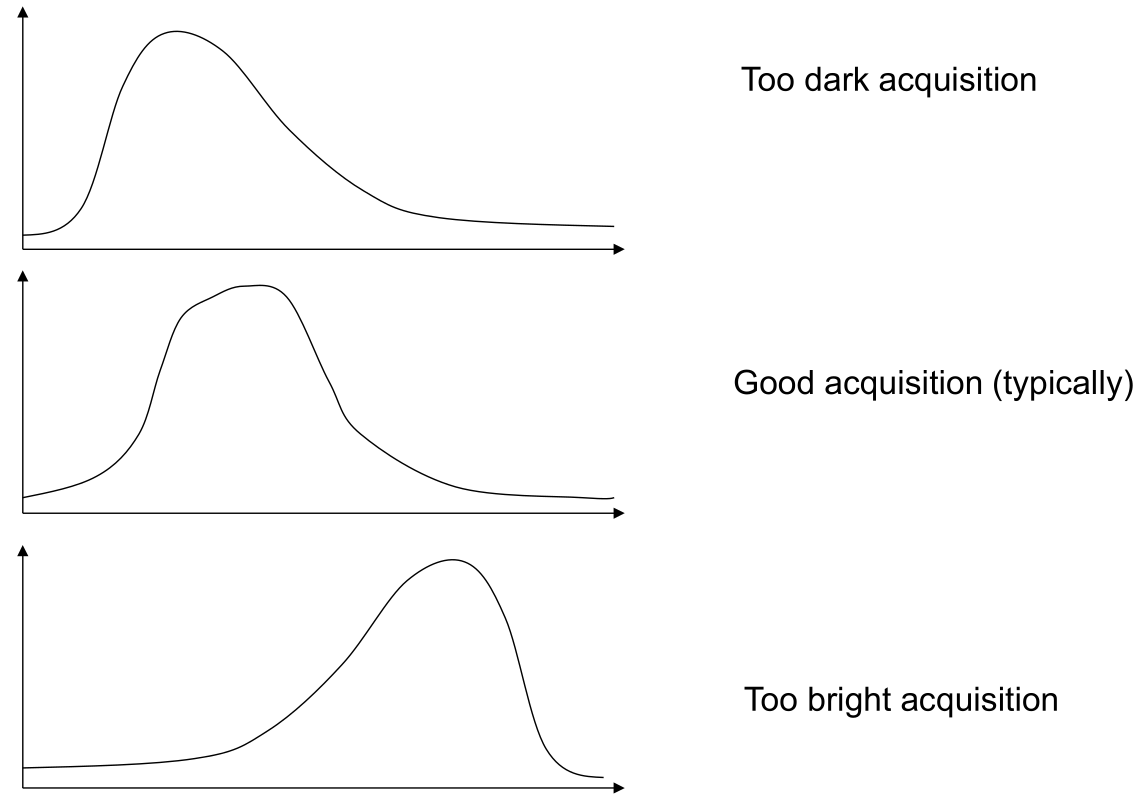
\includegraphics[width=.85\linewidth]{Picture/Histogram_Example}
\end{wrapfigure}
Semplicemente guardando la forma dell'istogramma ci si può rendere conto della bontà dell'immagine, o per lo meno della corretta esposizione. In un'immagine ci aspettiamo una distribuzione normale dai vari livelli di grigio, con pochi pixel che saturano il sensore in alto o in basso.

\begin{wrapfigure}[14]{l}{.4\linewidth}
	\vspace{-.3cm}
	\centering
	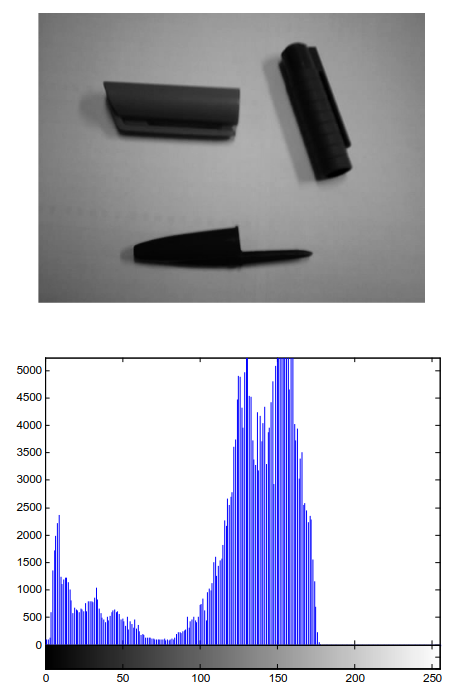
\includegraphics[width=.85\linewidth]{Picture/Histogram_Threshold}
\end{wrapfigure}
L'istogramma può inoltre essere utile per stimare la soglia di threshold più adatta a binarizzare un'immagine, infatti se siamo di fronte a un istogramma bimodale possiamo essere ragionevolmente certi che un picco rappresenti lo sfondo , mentre l'altro gli oggetti di nostro interesse. Tipicamente questa situazione si ritrova nei contesti di visione industriale e raramente nelle immagini naturali. Nell'immagine vediamo una situazione in cui è particolarmente evidente il valore che ci permette di avere una binarizzazione ragionevole dell'immagine; siamo quindi in una situazione molto favorevole.

\subsubsection{Equalizzazione dell'istogramma}
Una volta ottenuto l'istogramma di un immagine si può tentare di equalizzarlo in modo da migliorare l'immagine. Un istogramma concentrato solo su alcuni valori fa perdere dinamicità all'immagine, può quindi avere senso cercare di ripristinare una distribuzione uniforme dei valori dei pixel. Alla fine dell'equalizzazione vorremmo essere in una situazione come quella mostrata in figura qui sotto.

\begin{wrapfigure}[19]{r}{.45\linewidth}
	\vspace{-.4cm}
	\centering
	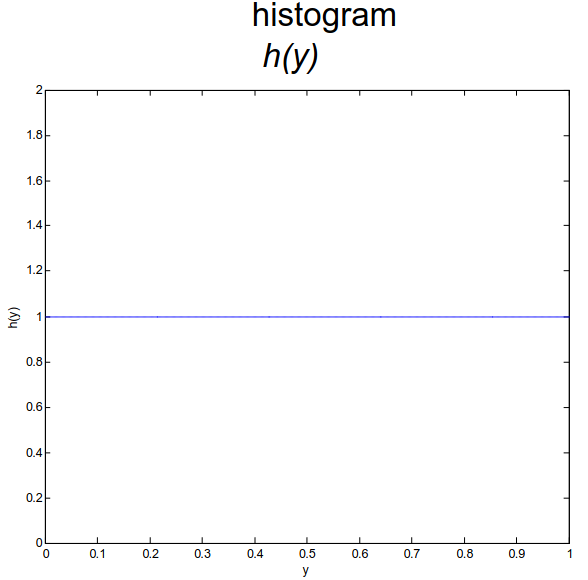
\includegraphics[width=.9\linewidth]{Picture/Histogram_EQ1}
	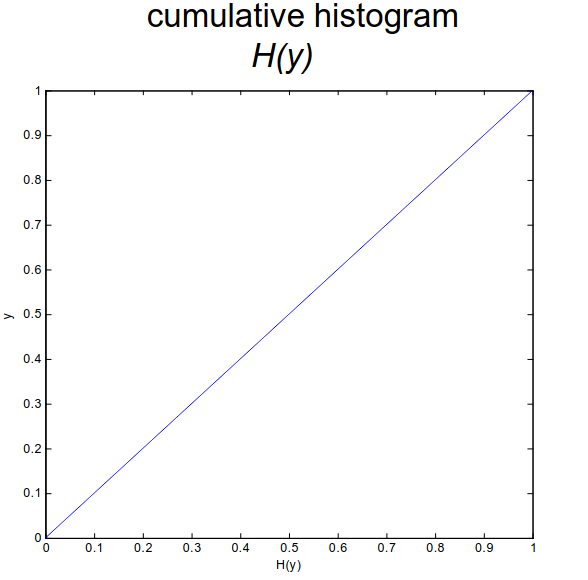
\includegraphics[width=.9\linewidth]{Picture/Histogram_EQ2}
\end{wrapfigure}
Per ottenere questo risultato consideriamo l'istogramma dell'immagine: $h(r)$ che associa a ogni livello di grigio $r$ il numero di pixel con quel valore. Definiamo l'istogramma cumulativo
\begin{equation}
	H(r) = \sum_{i = 0}^{r} h(i)
\end{equation}
e la funzione di trasformazione
\begin{equation}
	T(r) = (L - 1) \cdot \frac{H(r)}{M \cdot N}
\end{equation}
Dove $L$ è il numero di livelli di grigio, e $M$ e $N$ sono le dimensioni dell'immagine. Infine per ottenere l'immagine equalizzata trasformiamo ciascun pixel con
\begin{equation}
	y(i,j) = T[x(i,j)]
\end{equation}
Applicando queste trasformazioni possiamo ottenere un immagine con un istogramma equalizzato. È possibile che diversi livelli di grigio dell'immagine di partenza vengano mappati nello stesso livello di grigio dell'immagine di arrivo, è quindi necessari prestare attenzione alla possibile perdita di informazioni.

Si può costruire una trasformazione anche per ottenere una nuova immagine con un istogramma specificato, non per forza con distribuzione uniforme. Per fare questo costruisce $T$ che equalizza l'immagine di partenza, $G$ che equalizza l'istogramma che vogliamo ottenere, infine la trasformazione che permette di ottenere l'istogramma voluto sarà $z = G^{-1}(T(r))$.
\pagebreak
\section{Filtri}
\subsection{Caratteristiche generali}
I filtri permettono di applicare modifiche locali all'immagine e possono essere progettati sia nel dominio dello spazio che della frequenza. In questa prima e più semplice trattazione ci concentriamo sui filtri nel dominio dello spazio, indagando come certe caratteristiche dell'immagine possano essere messe in evidenza o nascoste a seconda di come progettiamo il filtro.

I filtri sono trasformazioni locali che si basano sulla \textbf{convoluzione} fra i pixel dell'immagine e una matrice che rappresenta il filtro stesso. Ci occuperemo di filtri:
\begin{itemize}
	\item Spazio invarianti;
	\item Lineari.
\end{itemize}
Date queste caratteristiche possiamo studiare l'effetto di un filtro semplicemente osservando la \textbf{risposta all'impulso}.  Siccome progetteremo sempre filtri 2D simmetrici fare la convoluzione sarà equivalente a sovrapporre la matrice quadrata che rappresenta il filtro all'immagine, moltiplicare i pixel per i pesi corrispondenti, sommare i risultati e immagazzinare il nuovo valore nel pixel centrale.

\subsection{Filtri passa-basso}
I filtri passa basso come suggerito dal nome sono filtri che eliminano le componenti a frequenza più alta, cioè si concentrano sui bordi dell'immagine sfumandoli.
\subsubsection{Media mobile}
\begin{wrapfigure}{r}{.5\linewidth}
	\vspace{-.3cm}
	\centering
	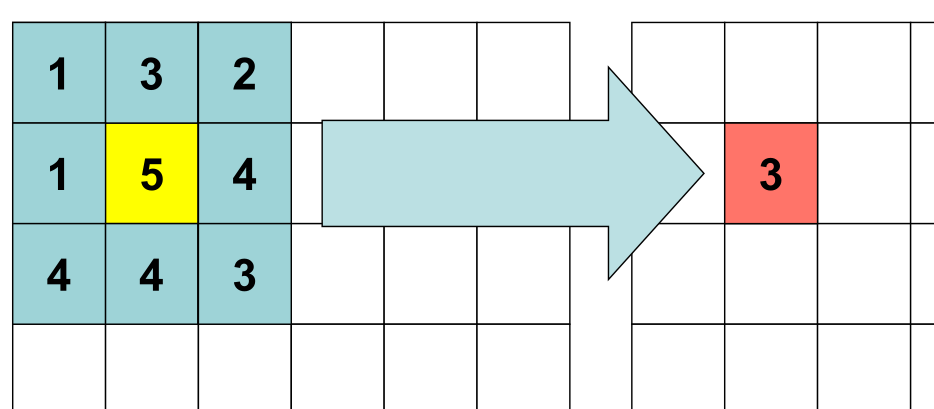
\includegraphics[width=.9\linewidth]{Picture/Moving_Average}
\end{wrapfigure}
Il più semplice filtro passa-basso e la media mobile, consiste nello scegliere una certa dimensione del filtro (\textbf{finestra}) e fare la media di tutti i pixel che si trovano nella finestra. Vedremo che un approccio di questo tipo può generare artefatti quando progetteremo filtri nel dominio della frequenza \ref{asd}.
\pagebreak
\subsubsection{Mediana}
\begin{wrapfigure}{l}{.6\linewidth}
	\centering
	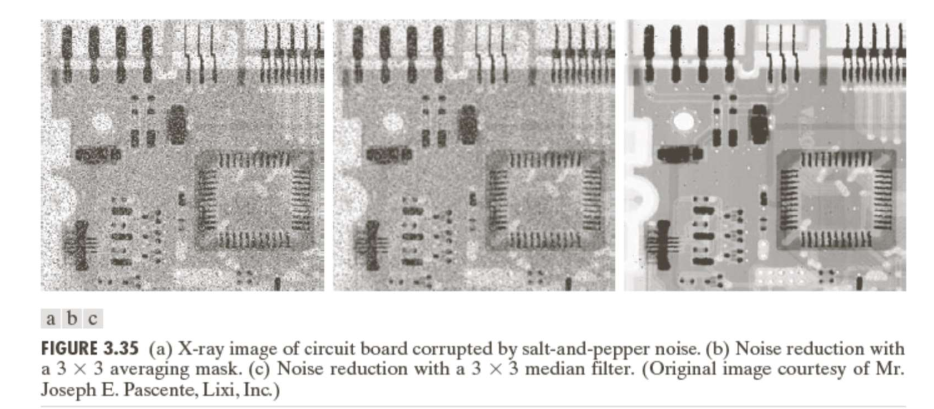
\includegraphics[width=.95\linewidth]{Picture/Median_Filter}
\end{wrapfigure}
Questo è un filtro non lineare, dato che la funzione che applica non è lineare, è comunque in filtro interessante dato che fa una statistica dei pixel all'interno della finestra e prende la mediana tra i pixel. Per questa ragione riesce a eliminare gli outlier che potrebbero essere presenti. Si comporta particolarmente bene per la rimozione del rumore sale e pepe.

\subsection{Filtri passa-alto}
I filtri passa alto servono per aumentare la nitidezza dell'immagine (\textbf{sharpening}) ed estrarre i bordi. Si ottengono cercando di calcolare le derivate dell'immagine, basandosi sull'idea che nei pressi dei bordi la derivata sarà elevata dato che c'è un cambio repentino nel valore dei pixel.
\subsubsection{Istogramma}
Prima di progettare dei filtri ad hoc proviamo ad applicare strumenti gia visti per aumentare il contrasto lungo i bordi. Possiamo ridefinire il concetto di equalizzazione in modo locale, andando considerare l'immagine costituita da sotto-immagini e equalizzando ciascuna parte in modo indipendente. Questo permette di aumentare il contrasto solo di alcune zone, ad esempio confrontando il valore medio dei pixel della zona con il valore medio dei pixel dell'immagine intera.
\subsubsection{Derivata dell'immagine}
Consideriamo la coordinata $x$ e definiamo la derivata nel caso discreto semplicemente come la differenza tra un campione e il successivo.
\begin{equation}
	\frac{\partial f}{\partial x} = f(x+1) - f(x)
\end{equation}
Data questa definizione possiamo applicare l'operatore derivata (che è lineare) alla derivata prima e ottenere la derivata seconda
\begin{equation}
	\frac{\partial^2 f}{\partial x^2} = f(x+1) + f(x-1) - 2 \cdot f(x)
\end{equation}
\subsubsection{Laplaciano}
Usando la derivata seconda possiamo costruire l'operatore laplaciano, questo operatore è invariante per rotazione e permette di aumentare la nitidezza dell'immagine.
\begin{wrapfigure}[14]{r}{.26\linewidth}
	\vspace{-.4cm}
	\centering
	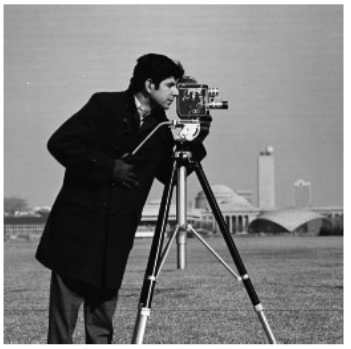
\includegraphics[width=.9\linewidth]{Picture/Cameraman_Original}
	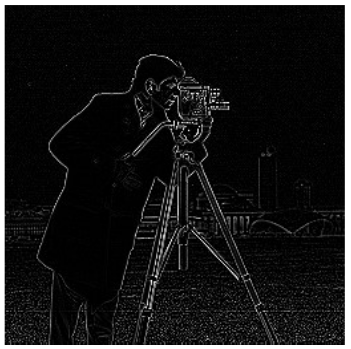
\includegraphics[width=.9\linewidth]{Picture/Cameraman_Laplacian}
\end{wrapfigure}
Definiamo il laplaciano come:
\begin{equation}
	\nabla^2 f = \frac{\partial^2 f}{\partial x^2} +  \frac{\partial^2 f}{\partial y^2}
\end{equation}
Possiamo ottenere un'immagine più nitida applicando la trasformazione
\begin{equation}
	g(x,y) = f(x,y) + c\cdot \nabla^2 f(x,y)
\end{equation}
Dove $c$ è un parametro che normalmente vale $\pm 1$.

Nell'immagine si vede il risultato del laplaciano applicato all'immagine (non è stato fatto sharpening, è solo stato applicato l'operatore $\nabla ^2$).
\subsubsection{Gradiente}
Considerando la derivata prima possiamo definire il gradiente dell'immagine in un dato pixel. Il gradiente è un vettore con una sua direzione e modulo. Possiamo usare il gradiente per costruire filtri che mettano in evidenza i bordi dell; immagine, dato che il gradiente ha una direzione possiamo considerare solo alcune componenti per enfatizzare i bordi orizzontali, verticali od obliqui; Oppure possiamo sommare tutte le componenti per evidenziare tutti i bordi.
\begin{wrapfigure}[7]{l}{.26\linewidth}
	\vspace{-.4cm}
	\centering
	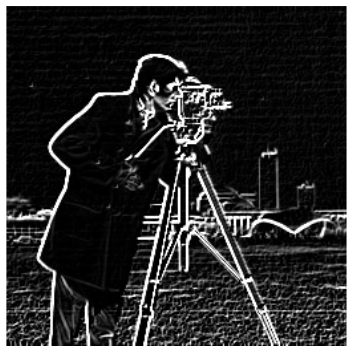
\includegraphics[width=.9\linewidth]{Picture/Cameraman_Gradient}
\end{wrapfigure}
Il gradiente è definito come:
\begin{equation}
	\nabla f = \frac{\partial f}{\partial x} \vec{i} +  \frac{\partial^2 f}{\partial y^2} \vec{j}
\end{equation}
Ed è sempre ortogonale alla direzione dei bordi dell'immagine. Se consideriamo solo le componenti orizzontali o verticali possiamo costruire gli operatori di Sobel mostrati qui sotto.
\begin{equation}
	S_x = 
	\begin{bmatrix}
		-1 & -2 & -1 \\
		0 & 0 & 0 \\
		1 & 2 & 1 
	\end{bmatrix}
	\quad \quad \quad
	S_y = 
	\begin{bmatrix}
		-1 & 0 & 1 \\
		-2 & 0 & 2\\
		-1 & 0 & 1 
	\end{bmatrix}
\end{equation}
L'immagine di esempio è stata ottenuta sommando il risultato dei due operatori di Sobel che evidenziano rispettivamente bordi orizzontali e verticali.

\section{Combinare gli strumenti}
Tutti gli strumenti presentati possono essere applicati in cascata per ottenere l'immagine desiderata. Ogni trasformazione ha lo scopo di semplificare il lavoro degli operatori a valle.
\begin{center}
	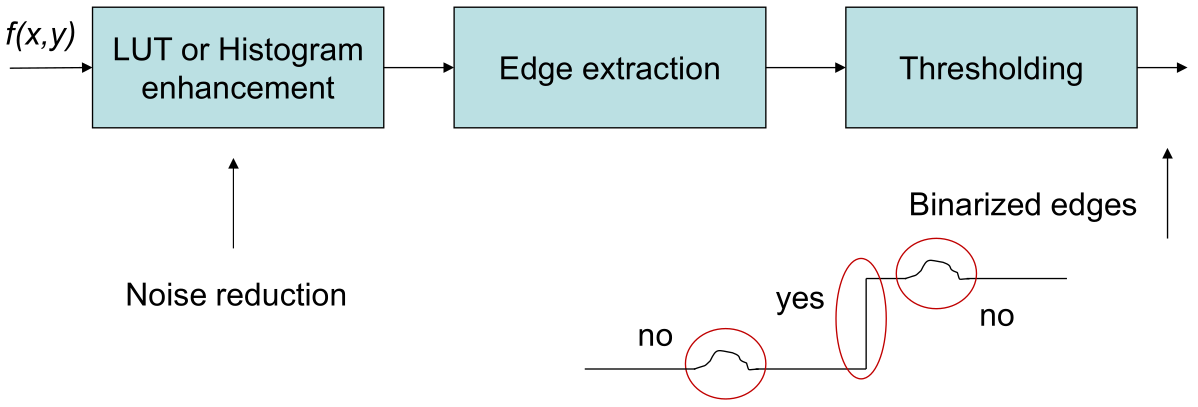
\includegraphics[width=.9\linewidth]{Picture/Enhancement_Pipeline}
\end{center}
Nell'immagine si vede una tipica pipeline di elaborazione di un'immagine, ovviamente ogni passaggio è optional e la sua applicazione o meno dipende dall'immagine di partenza, ma soprattutto dal risultato che si vuole ottenere; ricordando che l'enhancement è application-driven.
\chapter{Processing di immagini a colori}
Tutti gli strumenti presentati nel capitolo precedente possono essere applicati con successo anche alle immagini a colori, occorre però prestare attenzione e scegliere con giudizio come trattare i diversi canali. In \ref{sec:color_model} abbiamo presentato diversi spazi colore, scegliere quello corretto per rappresentare i dati che vogliamo elaborare è fondamentale ai fini di ottenere un buon risultato.

\section{Color slicing}
Avere a disposizione un'immagine colorata ci permette di segmentare l'immagine non solamente considerando l'energia totale (valore del livello di grigio), ma anche in base al colore.

\subsection{Segmentare col modello HSI}
Il modo più ovvio per segmentare un'immagine è quello di passare al modello HSI, in questo modello infatti possiamo definire direttamente la tinta (H) che ci interessa e selezionare tutti i pixel che hanno una tinta vicina.

In certi casi può essere utile avere delle soglie anche sulla saturazione (S), in modo da avere degli algoritmi robusti quando si dovessero incontrare colori la cui tinta non è ben definita come i grigi. Mentre non si usa mai l'intensità che non porta alcuna informazione sul colore.

Quando si segmenta con questo spazio colore è necessario prestare attenzione alla definizione del modello stesso, siccome la hue è la distanza dal rosso in corrispondenza del rosso c'è un salto di continuità, questo significa che tinte percettivamente simili al rosso come il magenta avranno in realtà distanza massima da quest'ultimo. Se si devono segmentare oggetti rossi bisogna prendere in considerazione questa discontinuità.

\subsection{Segmentare col modello RGB}
Per segmentare con lo spazio colore RGB abbiamo bisogno di definire il colore medio degli oggetti che vogliamo evidenziare, il modo più comodo per fare questo è selezionare a mano un certo numero di pixel che sappiamo appartenere all'oggetto di interesse e computare poi la media.

Una volta stabilito il colore medio abbiamo bisogno di un modo per accettare o rifiutare altri colori. Nello spazio HSI questo era molto semplice, si definiva una soglia e si valutava se la distanza dalla tinta selezionata era maggiore o minore. Nel modello RGB invece possiamo definire una distanza geometrica tra il colore del pixel che stiamo analizzando e il colore target (questo perché i colori si trovano in un cubo).

Abbiamo tipicamente tre alternative per decidere se accettare o meno un pixel:
\begin{itemize}
	\item \textbf{cubo}: costruiamo un cubo intorno al colore target, tutti i pixel il cui colore cade dentro al cubetto saranno selezionati;
	\item \textbf{sfera}: si definisce una distanza di soglia, tutti i pixel il cui colore dista da quello target meno della soglia saranno accettati;
	\item \textbf{distanza di Mahalanobis}: è una distanza adattativa che tiene conto che alcune componenti di colore possano variare più di altre.
\end{itemize}

\subsubsection{Distanza di Mahalanobis}
Usare una sfera per segmentare prevede che ciascuna componente possa variare fino a una soglia massima uguale per tutte le componenti. Ci sono casi in cui la componente verde del target rimane molto stabile mente la componente rossa varia molto, usare un sfera in questo caso porterà per forza a errori.

Quando si selezionano i pixel target si calcola anche una matrice di covarianza, questa ci permette di descrivere il comportamento di una componente rispetto alle altre e genera un'area di accettazione dei pixel a forma di ellissoide ruotato in modo da rispettare la distribuzione dei pixel che abbiamo selezionato per definire il colore target.

\begin{wrapfigure}{l}{.6\linewidth}
	\centering
	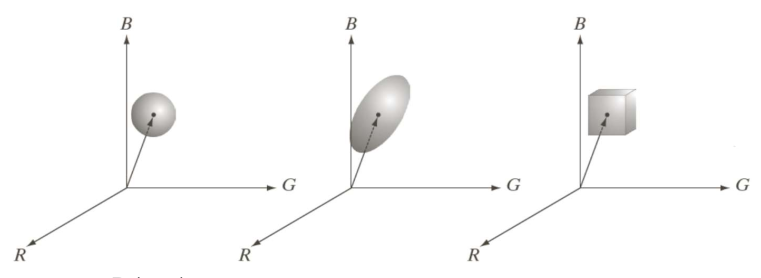
\includegraphics[width=.95\linewidth]{Picture/Color_Slicing}
\end{wrapfigure}
Nella figura sono rappresentate le diverse forme per definire la regione di accettazione dei pixel. Solo la distanza di Mahalanobis si adatta alla distribuzione dei pixel target.
\chapter{Enhancement con Fourier}
\section{Trasformata di Fourier continua}
Una funzione arbitraria può essere riscritta come l'integrale in frequenza di funzioni goniometriche elementari (seni e coseni) opportunamente pesati. Questo permette di passare da un dominio spaziale, quello dei campioni del segnale, al dominio di Fourier.

Scriviamo la trasformata di Fourier (FT) indicata con $F$ per un segnale monodimensionale. Considerando tempo $t$ e frequenze $\omega$ continue, è possibile derivare la trasformata di una funzione $f(t)$ (scriviamo $\mathfrak{F}$ per indicare che vogliamo calcolare la traformata di una funzione):
\begin{equation}
	\mathfrak{F}(f(t)) = F(\omega) = \int_{-\infty}^{\infty}f(t)e^{-i2\pi\omega t} dt
\end{equation}
e la sua inversa:
\begin{equation}
	\mathfrak{F}^{-1}(F(\omega)) = f(t) = \int_{-\infty}^{\infty} F(\omega)e^{i2\pi\omega t} d\omega
\end{equation}
Siccome cambia solo il segno dell'esponenziale possiamo derivare la proprietà di \textbf{simmetria}\label{prop:symmetryFT}: se $F(\omega)$ è la trasformata di $f(t)$ allora $f(-\omega)$ è la trasformata di $F(t)$.
\subsection{Trasformate notevoli}
\subsubsection{Impulso}
L'impulso è un segnale che vale 1 in zero e 0 in ogni altro istante. La sua trasformata sarà:
\begin{equation}
	F(\omega) = \int_{-\infty}^{\infty}\delta(t)e^{-i2\pi\omega t} dt = e^{-i2\pi\omega 0} = 1
\end{equation}
Questo significa che l'impulso contiene tutte le frequenze, inoltre ricordando le proprietà della trasformata (\ref{prop:symmetryFT}) la trasformata di una funzione costante è un impulso.

\subsubsection{Gradino}\label{sec:gradino}
\begin{wrapfigure}[7]{r}{.26\linewidth}
	\vspace{-1cm}
	\centering
	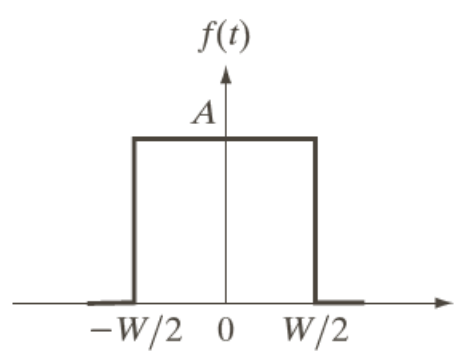
\includegraphics[width=.9\linewidth]{Picture/Step}
	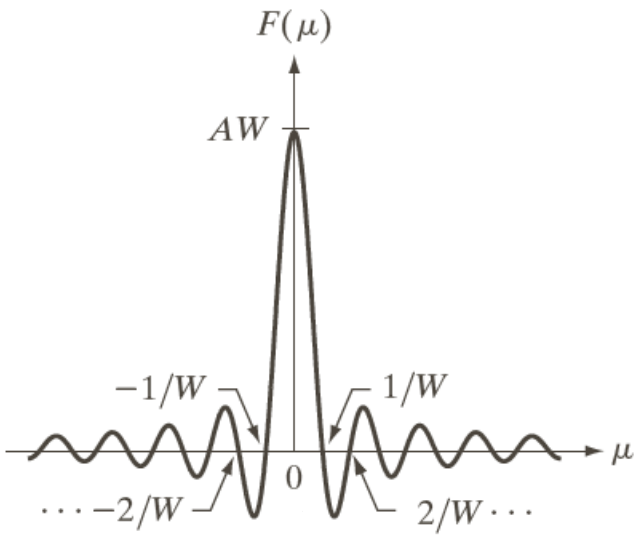
\includegraphics[width=.9\linewidth]{Picture/Sinc}
\end{wrapfigure}
Per una funzione a gradino, definita cioè da:
\begin{equation}
	f(t) = 
	\begin{cases}
		A & if -W/2 \leq t \leq W/2\\
		0 & otherwise
	\end{cases}
\end{equation}
La trasformata è un seno cardinale, cioè
\begin{equation}
	F(\omega) = AW \frac{\sin(\pi\omega W)}{\pi\omega W} = AW\text{sinc}(\omega W)
\end{equation}
\vspace{-.2cm}
\subsubsection{Coseno}
La trasformata del coseno è una coppia di impulsi centrati nell'origine che si trovano uno in $\omega$ (la frequenza del coseno), l'altro in $-\omega$

\subsubsection{Treno di impulsi}
\begin{wrapfigure}[5]{l}{.45\linewidth}
	\vspace{-.7cm}
	\centering
	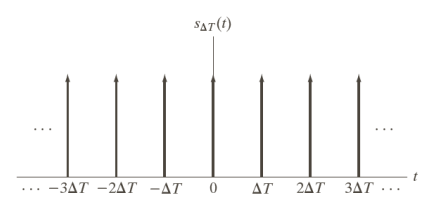
\includegraphics[width=.9\linewidth]{Picture/Impulse_Train}
\end{wrapfigure}
La trasformata di un treno di impulsi è nuovamente un treno di impulsi, se ogni impulso arriva dopo un tempo $\Delta T$, gli impulsi della trasformata si trovano a una distanza di $\frac{1}{\Delta T}$

\subsubsection{Funzioni pari e dispari}
Per le proprietà degli esponenziali una funzione pari trasformata rimane pari e una dispari rimane dispari. Lo stesso vale per l'antitrasformata, che preserva la parità della funzione di partenza.

\subsubsection{Funzioni traslate}
Considero una funzione $f(t)$, la sua trasformata $F(\omega)$ e una traslazione di $t_0$.  Si ottiene
\begin{equation}
	\begin{split}
		\mathfrak{F}(f(t-t_0)) &= \int_{-\infty}^{\infty} f(t - t_0)  e^{-i2\pi\omega t} dt = \\
		&=\int_{-\infty}^{\infty} f(s)  e^{-i2\pi\omega (s + t_0)} ds =\\
		& =e^{-i2\pi\omega t_0} \int_{-\infty}^{\infty} f(s)  e^{-i2\pi\omega s} ds =\\
		&=e^{-i2\pi\omega t_0}F(\omega)
	\end{split}
\end{equation} 
Il risultato è  ottenuto con la sostituzione di variabile $s = t - t_0 \rightarrow t = s + t_0$.

\subsection{Convoluzione}
La convoluzione è una funzione binaria $*$ che si applica a due funzioni $f(t)$ e $h(t)$. La sua definizione è:
\begin{equation}
	f(t)*h(t) = \int_{-\infty}^{\infty} f(\tau) \cdot h(t - \tau) d\tau
\end{equation}
Ricordando il risultato appena ottenuto della trasformata di funzioni traslate possiamo calcolare la trasformata della convoluzione ottenendo:
\begin{equation}
	\mathfrak{F}(f(t) * h(t)) = F(\omega)\cdot H(\omega)
\end{equation}
Cioè la covoluzione diventa un prodotto nel dominio trasformato. Similmente la convoluzione nel dominio di Fourier diventa un prodotto nel dominio del tempo. Questo risultato prende il nome di \textbf{teorema della convoluzione}.

\section{Sampling e DTFT}
Quando acquisiamo digitalmente un segnale, che sia mono o bi dimensionale lo stiamo campionando, è come se lo osservassimo solo in certi momenti. Possiamo quindi vedere il segnale campionato come il segnale originale moltiplicato per un treno di impulsi. La sua trasformata sarà quindi la convoluzione delle trasformate. Chiamiamo questa trasformata DTFT cioè Trasformata di Fourier a tempi discreti e la indichiamo con $\tilde{F}$.
\begin{equation}
	\tilde{F}(\omega) = F(\omega) * S(\omega) = \frac{1}{\Delta T} \sum_{n = -\infty}^{\infty} F(\omega - \frac{n}{\Delta T})
\end{equation}
Dove $S(\omega)$ è la trasformata del treno di impulsi che usiamo per il campionamento (sampling) e, di conseguenza, $\frac{1}{\Delta T}$ è la frequenza di campionamento. Otteniamo cioè infinite copie della trasformata della funzione originale, ciascuna traslata dalla precedente di $\frac{1}{\Delta T}$. 
\subsection{Teorema del campionamento}
Per fare in modo di riuscire a ricostruire fedelmente il segnale di partenza devo fare in modo che le varie copie non si intersechino (sommandosi); significa cioè che la frequenza di campionamento deve essere almeno doppia della frequenza massima presente nel segnale. Questo risultato è noto come \textbf{teorema del campionamento} o di Nyquist-Shannon.

Purtroppo per garantire che le frequenze presenti in un segnale siano limitate questo deve avere durata infinita, dato che questo non può mai verificarsi saremo costretti ad accettare un minimo di sovrapposizione.

\subsection{Aliasing}
Quando le copie della trasformata si sovrappongono si verifica il fenomeno dell'aliasing, ovvero le frequenze più alte del segnale originale vanno ad alterare le frequenze più basse del segnale ricostruito. L'unica soluzione per poter ricostruire il segnale originale è quindi quella di aumentare la frequenza di campionamento.

Quando non è possibile modificare il processo di acquisizione del segnale si possono applicare (prima dell'acquisizione) dei filtri per limitare le frequenze più alte (filtri passa basso).  Questi filtri sono detti anti aliasing, modificheranno il segnale, che non sarà più quello originale, ma spesso questa alterazione è molto minore dell'aliasing. 
\begin{center}
	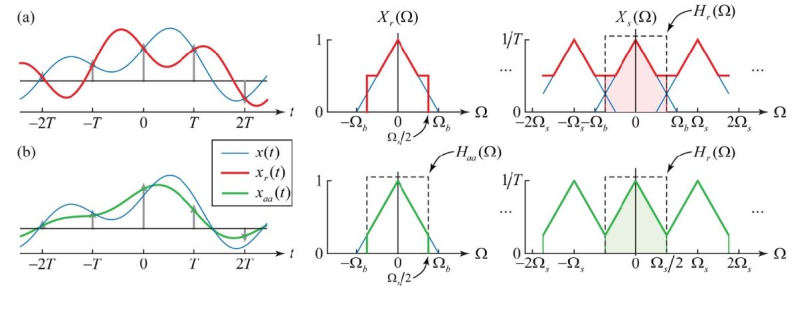
\includegraphics[width=.9\linewidth]{Picture/Aliasing}
\end{center} 
\vspace{-.3cm}
 L'immagine mostra sengale originale (azzurro), ricostruito e trasformata in assenza (a) e presenza (b) di filtri anti alaising, si vede bene come il segnale verde  si avvicini di più all'originale del segnale rosso.
 
 \section{Trasformata di Fourier Discreta}
 Prima abbiamo considerato la trasformata di un segnale a tempi discreti, ora proviamo a discretizzare anche le frequenze e per fare questo consideriamo la periodicità della trasformata $\tilde{F}$ e la campioniamo per un periodo ottenendo M campioni. Si può allora ottenere la Trasformata di Fourier discreta DFT (sia nel dominio dello spazio che della frequenza):
 \begin{equation}
 	F(m) = \sum_{x = 0}^{M-1} f(x)e^{\frac{-i2\pi m x}{M}}
 \end{equation}
 e la sua inversa:
  \begin{equation}
 	f(x) =\frac{1}{M} \sum_{m = 0}^{M-1} F(m)e^{\frac{i2\pi m x}{M}}
 \end{equation}
 Dove sia $x = 0,  1,\dots, M$ che $m = 0,  1,\dots, M$ sono intere e rappresentano rispettivamente gli istanti discreti di tempo e le frequenze discrete.

È facile mostrare che sia la trasformata che l'inversa sono periodiche di periodo $M$. È possibile interpretare la trasformata di Fourier come un cambio di base che ci permette di passare dal dominio spaziale al dominio temporale tramite una matrice di trasformazione (il kernel della trasformata).

\section{Trasformata 2D continua}
Possiamo estendere il concetto di trasformata Fourier al caso bidimensionale ottenendo le seguenti espressioni:
\begin{equation}
	\mathfrak{F}(f(t,z)) = F(u,v) = \int_{-\infty}^{\infty}\int_{-\infty}^{\infty} f(t, z)  e^{-i2\pi (ut + vz)} dt dz
\end{equation}
\begin{equation}
	\mathfrak{F}^{-1}(F(u,v)) = f(t,z) = \int_{-\infty}^{\infty}\int_{-\infty}^{\infty} F(u,v)  e^{i2\pi (ut + vz)} du dv
\end{equation}
Notiamo che siccome le variabili sono indipendenti posso l'integrale è separabile, quindi è possibile integrare prima su una variabile poi sull'altra.

\section{Sampling 2D}
Possiamo ripetere i ragionamenti fatti nel caso monodimensionale quando passiamo al caso bidimensionale. In 2D per campionare non usiamo un treno di impulsi ma una matrice e possiamo ottenere tutti i risultati del caso 1D.
\subsection{Teorema del campionamento}
Possiamo essere sicuri di ricostruire fedelmente un segnale se lo campioniamo a una frequenza almeno doppia della frequenza massima presente nel segnale. Siccome usiamo per acquisire un sensore rettangolare che rappresenta la matrice di impulsi possiamo considerare separatamente frequenze verticali e orizzontali.
\subsection{Aliasing 2D}
Solo funzioni illimitate nel dominio dello spazio sono limitate nel dominio della frequenza, e viceversa, quando acquisiamo un'immagine o un video questo sarà per forza limitato nello spazio e nel tempo, questo porta ad avere un segnale a banda illimitata.

Per quanto detto prima la frequenza di acquisizione sarà sicuramente minore della frequenza massima presente nel segnale. Per limitare il fenomeno dell'aliasing sarà quindi necessario applicare dei filtri passa basso prima dell'acquisizione.
\subsubsection{Aliasing e scalamento}
\begin{wrapfigure}{l}{.63\linewidth}
	\vspace{-.5cm}
	\centering
	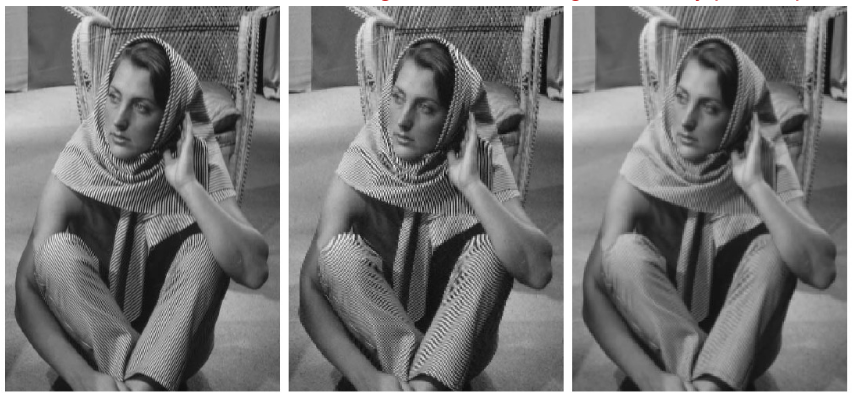
\includegraphics[width=\linewidth]{Picture/Aliasing_Scaling}
\end{wrapfigure}
Quando riduciamo le dimensioni dell'immagine non è sufficiente prendere un pixel ogni due od ogni tre, perché in questo modo si riduce la frequenza di campionamento senza ridurre le frequenze presenti nell'immagine, quindi potrebbero presentarsi artefatti dovuti al rimpicciolimento. Per evitare questo fenomeno è necessario, prima di fare lo scalamento applicare un filtro di blurring che elimini le frequenze troppo alte dall'immagine. Nell'immagine si vede l'immagine originale seguita da un esempio di scalamento prima senza filtro e poi con filtro che elimina le Moirè

\section{Trasformata 2D discreta}
Vediamo ora l'effetto del campionamento sulla trasformata di Fourier:
\begin{equation}
	F(u,v) = \sum_{x=0}^{M-1}\sum_{y=0}^{N-1}f(x,y) e^{-i2\pi (\frac{ux}{M} + \frac{vy}{N})}
\end{equation}
e la sua inversa: 
\begin{equation}
	f(x,y) = \frac{1}{MN}\sum_{u=0}^{M-1}\sum_{v=0}^{N-1}F(u,v) e^{i2\pi (\frac{ux}{M} + \frac{vy}{N})}
\end{equation}
Dove la distanza spaziale tra due campioni orizzontali è $\Delta T$ e tra due campioni verticali è $\Delta Z$, mentre la separazione tra due frequenze orizzontali e verticali è rispettivamente $\Delta u = \frac{1}{M \Delta T}$ e $\Delta v = \frac{1}{N \Delta Z}$

\subsubsection{Modulo e fase}
Come nel caso monodimensionale anche in 2D la trasformata di un \textbf{segnale reale} ha modulo pari e fase dispari.

Se proviamo a fare il plot della fase spesso ci troviamo di fronte un'immagine che pare di puro rumore, nonostante questo è la fase che trasporta le informazioni sulla forma dell'immagine, provando a ricostruire un'immagine solo con la fase si riesce ancora spesso a capire il soggetto, è impossibile invece con il modulo.

\subsection{Traslazioni e rotazioni}
\begin{wrapfigure}{l}{.3\linewidth}
	\vspace{-.5cm}
	\centering
	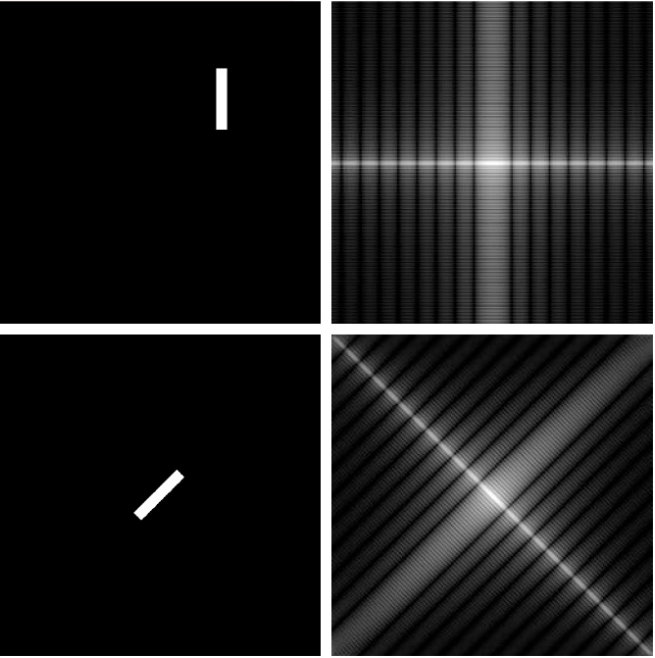
\includegraphics[width=.95\linewidth]{Picture/Rotation_Traslation}
\end{wrapfigure}
La trasformata di Fourier è invariante per traslazione, mentre ruotare l'immagine significa ruotare la trasformata e ruotare la trasformata significa ruotare l'antitrasformata (l'immagine). Nell'esempio si vede prima il rettangolo bianco traslato in alto a destra, che non altera la trasformata, poi il rettangolo ruotato che ha come effetto la rotazione della trasformata.

\subsection{Convoluzione 2D}
In due dimensionei la convoluzione è definita come:
\begin{equation}
	f(x,y) * h(x,y) = \sum_{m=0}^{M-1}\sum_{n=0}^{N-1} f(m,n) h(x-m, y-n)
\end{equation}
Si può dimostrare il \textbf{teorema della convoluzione 2D} che afferma che cambiando dominio la convoluzione diventa un prodotto e viceversa, formalmente si ha che:
\begin{equation}
	f(x,y)*h(x,y)  \Longleftrightarrow F(u,v)H(u,v)
\end{equation}
\begin{equation}
	f(x,y)h(x,y)  \Longleftrightarrow F(u,v)*H(u,v)
\end{equation}

\section{Filtraggio nel dominio della frequenza}
L'idea di base è quella di passare al dominio della frequenza per poter moltiplicare la trasformata del segnale con la trasformata del filtro, poi tornare al dominio spaziale per ottenere il risultato.

\subsection{Zero Padding}
Siccome quando facciamo la trasformata di un segnale 2D di dimensione $N\times M$ otteniamo una trasformata con le stesse dimensioni e per moltiplicare due sengali o due trasformate è necessario che entrambi abbiano le stesse dimensioni dobbiamo fare in modo che i segnali di partenza abbiano la stessa dimensione. Per fare questo possiamo fare \textbf{zero padding}m cioè aggiungere alle funzioni (segnali) degli zeri, in modo che abbiano la stessa dimensione.

Aggiungere degli zeri alla fine di una funzione può però generare componenti di alta frequenza, dato che sarebbe come moltiplicare il segnale per una finestra rettangolare, che abbiamo visto avere un seno cardinale come trasformata (\ref{sec:gradino}); questo fenomeno si chiama \textbf{frequency leakage}.

Per mitigare il frequency leakage al posto che moltiplicare la funzione per un gradino si usano finestre più morbide, che vanno a zero senza salti netti; le finestre più usate sono Gaussiana, di Hann, di Hamming, di Barlett.

\subsection{Progettare un filtro}
Passare al dominio della frequenza ci permette di progettare i filtri in modo nuovo, concentrandoci sulle frequenze e i pattern che vogliamo eliminare dall'immagine.

Purtroppo quando operiamo nel dominio della frequenza dovremmo evitare di creare filtri ideali, dato che questi si traducono in filtri di dimensione infinita nel dominio dello spazio e portano al frequency leakage.

Inoltre quando progettiamo un filtro non vogliamo andare a deformare l'immagine di partenza, dato che l'informazione sulle forme è portata dalla fase della trasformata vorremmo che il filtro non alteri la fase.

In generale quando progettiamo un filtro per un'immagine $f(x,y)$ di dimensioni $M\times N$ dovremmo seguire i seguenti passaggi, che nella maggior parte delle applicazioni portano a dei risultati accettabili:
\begin{enumerate}
	\item fare zero padding dell'immagine arrivando alla dimensione $P\times Q = 2M\times 2N$
	\item moltiplicare l'immagine per $(-1)^{x+y}$ in modo da centrare la trasformata nell'origine
	\item calcolare la trasformata $F(u,v)$
	\item generare il filtro $H(u,v)$ di dimensioni $P\times Q$ centrato in $P/2, Q/2$
	\item calcolare la trasformata del risultato come $G(u,v) = H(u,v)F(u,v)$
	\item calcolare la parte reale dell'antitrasformata e traslarla nell'origine moltiplicando di nuovo per $(-1)^{x+y}$
	\item ritagliare l'immagine alla dimensione $M\times N$
\end{enumerate}
\chapter{Image Restoration}
L'image restoration è un processo oggettivo, che passa attraverso la modellazione del danneggiamento subito dall'immagine per poi correggerla. Si appoggia a delle metriche per stabilire se è stato raggiunto l'ottimo nella curva di riparazione.

\begin{center}
	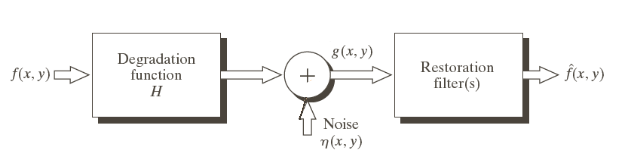
\includegraphics[width=.7\linewidth]{Picture/Restoration_Process}
\end{center}
In figura si vede un tipico processo di restoration: si parte dall'immagine originale ($f(x,y)$), perfetta, si passa attraverso un primo filtro che danneggia l'immagine (ad esempio la macchina non ha messo correttamente a fuoco), assumeremo che questo filtro sia lineare e spazio invariante. Durante il processo di acquisizione poi potrebbe essere sommato all'immagine del rumore (tipicamente pdovuto a imperfezioni del sensore) e si arriva all'immagine degradata ($g(x,y)$). All'immagine rovinata si possono applicare uno o più filtri di restoration per ottenere una stima dell'immagine originale ($\hat{f}(x,y)$).

Siccome Assumiamo che i filtri che rovinano l'immagine siano lineari e spazio invarianti possiamo scrivere 
\begin{gather}
	g(x,y) = h(x,y)*f(x,y) + \eta(x,y)\\
	G(u,v) = H(u,v)\cdot F(u,v) + N(u,v)
\end{gather}
Dove le lettere maiuscole indicano la trasformata di Fourier della funzione con la minuscola.

\section{Rumore}
È un danno all'immagine dovuto all'ambiente e alla tipologia di acquisizione dell'immagine. Possiamo studiarne le proprietà attraverso lo spettro in frequenza (ad esempio spettro piatto per il rumore bianco) e in generale assumiamo sia spazio invariante.

\subsection{Stimare il rumore}
Oltre al rumore bianco l'immagine può essere affetta da rumori distribuiti in molti modi. Per stimare i parametri del rumore si possono adottare diverse tecniche.
\subsubsection{Rumore spazio invariante} 
\begin{wrapfigure}[11]{r}{.3\linewidth}
	\vspace{-.8cm}
	\centering
	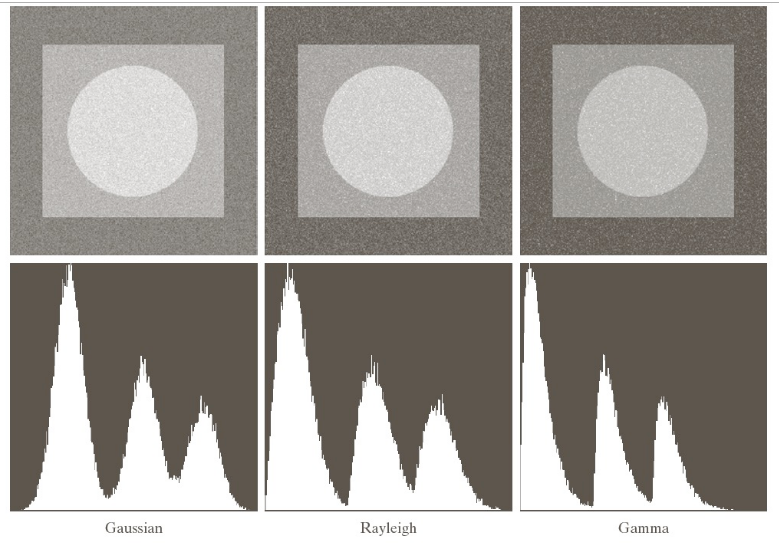
\includegraphics[width=.95\linewidth]{Picture/Noise_Distribution1}
	\\
	\vspace{.1cm}
	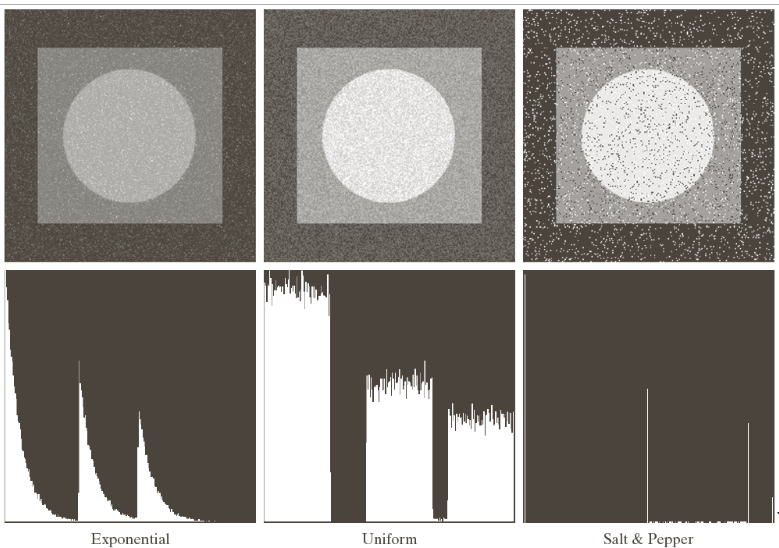
\includegraphics[width=.95\linewidth]{Picture/Noise_Distribution2}
\end{wrapfigure}
Siamo interessati a stimare la PDF del rumore, per fare questo si può considerare una zona dell'immagine che sappiamo avere uno stesso livello di grigio e studiare l'istogramma di quella zona, per osservare la distribuzione del rumore. Nelle immagini vediamo alcuni esempi di come differenti distribuzioni del rumore danneggiano immagini sintetizzate. Anche in questi esempi molto semplici è molto difficile capire il tipo di rumore senza guardare l'istogramma.

Capire la PDF del rumore è importante dato che sono stati ingegnerizzati  filtri apositi che, sfruttando le conoscenze a priori della PDF, correggono meglio i danni provocati da un certo tipo di rumore.

\subsubsection{Rumore spazio dipendente} 
\begin{wrapfigure}[9]{l}{.3\linewidth}
	\vspace{-.6cm}
	\centering
	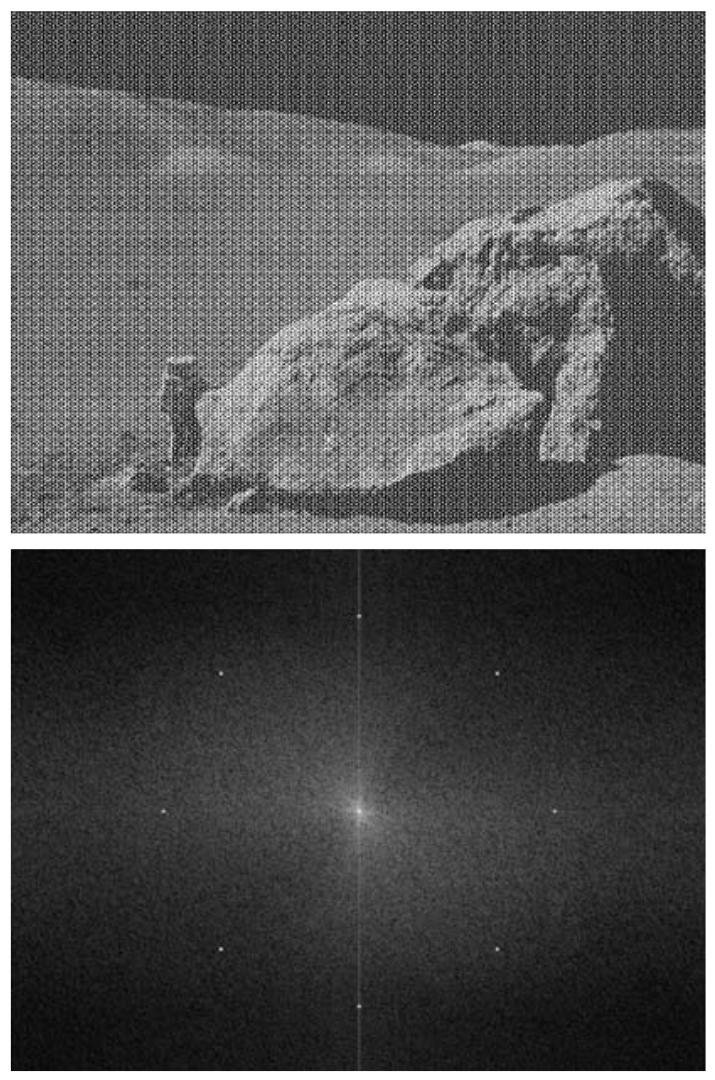
\includegraphics[width=.95\linewidth, height=4.5cm]{Picture/Periodic_Noise}
\end{wrapfigure}
Normalmente questo è dovuto al particolare processo di acquisizione, in questo caso ci concentriamo sul rumore periodico, che è un particolare tpo di rumore spazio dipendente. Il rumore periodico può essere individuato da dei picchi visibili nella trasformata di Fourier dell'immagine, è in questo domino che progettiamo i filtri per imuovere il rumore periodico. Ogni componente del rumore genera 2 picchi simmetrici nella trasformata.
\newpage

\section{Rumore spazio invariante}
Progettiamo dei \textbf{filtri nel dominio spaziale} per ridurre il rumore presente in un immagine. Questi filtri sono adatti quando nell'immagine è presente rumore additivo. Il modello di degradazione è:
\begin{gather}
	g(x,y) = f(x,y) + \eta(x,y)\\
	G(u,v) = F(u,v) + N(u,v)
\end{gather}
Nel prgettare questi filtri prenderemo in considerazione un pixel e i suoi vicini, questi possono essere disposti a croce, gli  8 tutti attorno oppure possiamo considerare un quadrato più grande, chiameremo $S_{xy}$ il vicinato (\textbf{neighbourhood}) del pixel a coordinate $(x,y)$
\subsection{Filtri semplici}
\subsubsection{Filtri che operano una media}
\begin{description}
	\item [Aritmetica] 
		\begin{equation}
			\hat{f} = \frac{1}{mn} \sum_{(s,t)\in S_{xy}} g(s,t)
		\end{equation}
		Il rumore è ridotto grazie al blurring, è l'unico filtro lineare (solo per questo ha senso studiare la risposta in frequenza);
	\item[Geometrica]
		\begin{equation}
			\hat{f} =\Bigg[\prod_{(s,t)\in S_{xy}} g(s,t)\Bigg]^{\frac{1}{mn}}
		\end{equation}
		Riduce il rumore ma preserva più dettagli rispetto alla media aritmetica;
	\item[Armonica]
		\begin{equation}
			\hat{f} = \frac{mn} {\sum_{(s,t)\in S_{xy}} \frac{1}{g(s,t)}}
		\end{equation}
		Adatta a ridurre il rumore gaussiano e di tipo sale, fallisce con il rumore pepe;
	\item[Contrarmonica]
		\begin{equation}
			\hat{f} = \frac{\sum_{(s,t)\in S_{xy}} g(s,t)^{Q+1}} {\sum_{(s,t)\in S_{xy}} g(s,t)^Q}
		\end{equation}
		$Q$ è l'ordine della media, se $Q>0$ adatta per rumore pepe, se $Q<0$ adatta per rumore sale, se $Q=0$ o $Q=-1$ si riade in media aritmetica o armonica rispettivamente.
\end{description}

\subsubsection{Filtri basati sull'ordinamento dei livelli d'intensità}
Questi filtri sono adatti alla rimozione degli outlier.
\begin{description}
	\item[Mediana]
		\begin{equation}
			\hat{f} = \underset{(s,t)\in S_{xy}}{\text{median}}\ g(s,t)
		\end{equation}
		Adatto a rimuovere rumore impulsivo, può rovinare i bori sottili;
		\item[Max/Min]
		\begin{equation}
			\hat{f} = \underset{(s,t)\in S_{xy}}{\text{max/min}}\ g(s,t)
		\end{equation}
		Adatti a rimuovere rispettivamente rumore pepe e sale;
		\item[Punto medio]
		\begin{equation}
			\hat{f} = \frac{\underset{(s,t)\in S_{xy}}{\text{max}}\ g(s,t) + \underset{(s,t)\in S_{xy}}{\text{min}}\ g(s,t)}{2}
		\end{equation}
		Adatto a rimuovere rumore casuale gaussiano o uniforme;
		\item[Alfa trimmed]
		\begin{equation}
			\hat{f} = \frac{1}{mn - d} \sum_{(s,t)\in S_{xy}} g'(s,t)
		\end{equation}
		Prima di calcolare la media vengono scartati i $d/2$ valori più piccoli e i $d/2$ valori più grandi. È adatto per rimuovere rumore sale e pepe e gaussiano assieme.
\end{description}

\subsection{Filtri adattativi}
Sono filtri che adattano il loro comportamento in base alle caratteristiche locali dell'immagine, tipicamente si considera una finestra $m\times n$ che rappresenta il vicinato di un pixel e si confrontano le caratteristiche della finestra con quelle dell'immagine intera per dosare il comportamento del filtro.
\subsubsection{Media adattativa}
	\begin{equation}
		\hat{f}(x,y) = g(x,y) - \frac{\sigma_{\eta}^2}{\sigma_L^2}[g(x,y) - m_L]
	\end{equation}
Dove $\sigma_{\eta}$ è la varianza del rumore, $\sigma_L$ è la varianza locale e $m_L$ è la media locale. La media locale rappresenta la luminanza nella zona che stiamo considerando, mentre la varianza locale il contrasto. 
\newpage
A seconda del rapporto tra la varianza del rumore e la varianza locale il filtro si comporta in modo diverso:
\begin{itemize}
	\item $\sigma_{\eta} = 0$ non c'è rumore quindi $\hat{f}(x,y) = g(x,y) = f(x,y)$;
	\item $\sigma_L \gg \sigma_{\eta}$ molto contrasto, ci sono dei bordi, quindi non bisogna filtrare troppo per non rovinare i gettagli $\hat{f}(x,y) \approx g(x,y)$;
	\item $\sigma_L = \sigma_{\eta}$ la finestra ha le stesse caratteristiche dell'immagine, il filtro si comporta esattamente come la media;
	\item $\sigma_{\eta} > \sigma_L$ si forza $\sigma_{\eta} = \sigma_L$ per non ottenere dei valori negativi, questo potrebbe rendere necessario riscalare i valori dell'immagine per non perdere della dinamica dell'immagine.
\end{itemize}

Affinché questo filtro possa funzionare correttamente è essenziale avere una stima accurata della varianza del rumore.

\subsubsection{Mediana adattativa}
Questo filtro ha lo scopo di preservare i bordi, rimuovere il rumore impulsivo, fare smoothing del rumore random senza allargare o assottigliare i bordi.
\vspace{.5cm}

\begin{algorithmic}
	\Function{AdaptativeMedian}{ }
		\State $S_{xy} \gets S_{min}$
		\While{$S_{xy} \leq S_{max}$}
			\State $A_1 \gets z_{med} - z_{min}$
			\State $A_2 \gets z_{med} - z_{max}$
			\If{$A_1 > 0 \textbf{ and } A_2 < 0$}
				\State $B1 \gets z_{xy} - z_{min}$
				\State $B1 \gets z_{xy} - z_{max}$
				\If{$B_1 > 0 \textbf{ and } B_2 < 0$}
					\State \Return $z_{xy}$
				\Else
					\State \Return $z_{med}$
				\EndIf
			\Else
				\State $S_{xy} \gets$ \Call{IncrementNeighbourhood}{ }
			\EndIf
		\EndWhile
		\State \Return $z_{med}$
	\EndFunction    
\end{algorithmic}

Dove:
\begin{itemize}
	\item $S_{xy}$: Area del vicinato del pixel $(x,y)$;
	\item $z_{min}$: Intensità minima nell'area considerata;
	\item $z_{max}$: Intensità massima nell'area considerata;
	\item $z_{med}$: Intensità media nell'area considerata;
	\item $z_{xy}$: Intensità del pixel $(x,y)$;
	\item $S_{min}$:Area di partenza del vicinato;
	\item $S_{max}$: Massima area del vicinato consentita.
\end{itemize}

Come si vede questo filtro è in grado di modificare, entro certi limiti, la dimensione della finestra di vicinato. Il filtro calcola la mediana, se questa corrisponde al minimo o al massimo dell'intensità si aumenta la dimensione della finestra, altrimenti si decide se restituire la mediana o il valore del pixel. Si restituisce il valore del pixel se questo ha le stesse caratteristiche che abbiamo richiesto per la mediana (non è né un minimo né un massimo di intensità).

\section{Rumore spazio dipendente}
Progettiamo dei filtri \textbf{nel dominio della frequenza} per ridurre il rumore additivo spazio dipendente.
Per descrivere il rumore osserveremo quali sono le sue componenti nella trasformata di Fourier e cereremo di isolare l'immagine rispetto al rumore.

\subsection{Notch Filter}
Il rumore periodico si individua facendo la trasformata e cercando dei picchi nella stessa. Ogni componente genera 2 picchi simmetrici rispetto all'origine. Per rimuovere il rumore periodico si può usare un filtro \textbf{notch} $H_{NR}$. Questo è costituito dal prodotto di filtri passa alto centrati sui picchi di rumore.
\begin{equation}
	H_{NR}(u,v) = \prod_{k=1}^{Q} H_k(u,v) H_{-k}(u,v)
\end{equation}
Dove $ H_k(u,v)$ è il filtro passa alto centrato in $u_k,v_k$ e $H_{-k}(u,v)$ è il simmetrico rispetto all'origine.

Ciascun $H_k$ può essere costruito utilizzando diverse forme (ideale, gaussiano, butterworth, ecc\dots) indipendentemente dagli altri filtri passa alto, l'importante è che $H_{k}(u,v)$ e $H_{-k}(u,v)$ abbiano la stessa forma.

\begin{wrapfigure}{r}{.5\linewidth}
	\vspace{-.4cm}
	\centering
	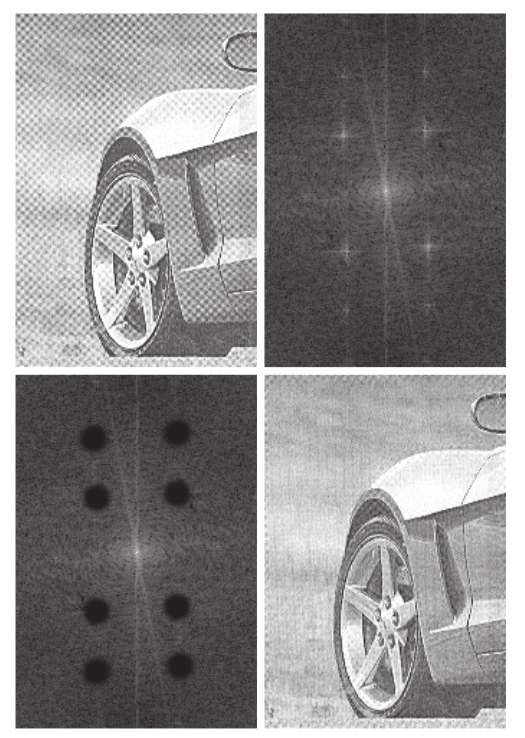
\includegraphics[width=.95\linewidth]{Picture/Notch}
\end{wrapfigure}
Per fare image enanchement è sufficiente centrare i filtri passa alto nei picchi di rumore visibili nella trasformata di Fourier e filtrare l'immagine utilizzando il filtro notch ottenuto componendo i passa alto. Il risultato che si ottiene è spesso più soddisfacente rispetto all'immagine che si otterrebbe con dei filtri di blurring. Inoltre se i picchi di rumore sono sufficientemente distanti dalle frequenze che caratterizzano l'immagine il filtro notch non rovina i dettagli, neppure quelli più fini. L'immagine mostra la situazione originale e l'applicazione dei filtri passa alto in corrispondenza dei picchi di rumore, come si vede il risultato è soddisfacente.

\subsubsection{Optimum Notch}
Costruiamo a partire dal filtro notch un filtro adattativo che pesi l'effetto del filtro notch a seconda delle caratteristiche locali dell'immagine. Come sempre consideriamo il vicinato $S_{xy}$ del pixel $(x,y)$ e ricaviamo un filtro che minimizzi la varianza locale dell'immagine ricostruita $\hat{f}(x,y)$. Per costruire l'optimum notch abbiamo bisogno di:
\begin{itemize}
	\item filtro che isoli il rumore: $H_{NP} = 1 - H_{NR}$
	\item rumore stimato: $\eta(x,y)= \mathfrak{F}^{-1}\{N(u,v)\}= \mathfrak{F}^{-1}\{H_{NP}(u,v)G(u,v)\}$
	\item immagine ricostruita: $\hat{f} = g(x,y) - w(x,y)\eta(x,y)$
\end{itemize}
Dove pesiamo il rumore con $w(x,y)$ perché non è il rumore esatto, ma solo una stima.

Siamo pronti per calcolare la varianza locale dell'immagine ricostruita; chiamiamo il valor medio di una misura come la misura stessa con una barretta sopra, ad esempio $\overline{\eta}$ è il valor medio del rumore nella finestra considerata.
\begin{align}
	&\sigma^2(x,y) = \frac{1}{mn} \sum_{(r,c)\in S_{xy}}\Big[\hat{f}(r,c) - \overline{\hat{f}}\Big] =	& \\
	&= \frac{1}{mn} \sum_{(r,c)\in S_{xy}} \Big\{ [g(c,r) -w(c,r)\eta(c,r)] - [\overline{g} -\overline{w\eta}]\Big\}^2 = & \text{def. di } \hat{f}  \notag \\
	&= \frac{1}{mn} \sum_{(r,c)\in S_{xy}} \Big\{ [g(c,r) -w(c,r)\eta(c,r)] - [\overline{g} - w(x,y)\overline{\eta}]\Big\}^2 & \qquad\overline{w}= w(x,y)  \notag
\end{align}
Nell'ultimo passaggio approssimo i pesi della finestra al peso del pixel centrale ($w(c,r) = w(x,y)$), quindi la media sarà il peso del pixel centrale. 

Possiamo derivare la varianza in funzione di $w(x,y)$ e imporla a $0$, si ottiene il vincolo su $w(x,y)$:
\begin{equation}
	w(x,y) = \frac{\overline{g\cdot\eta} - \overline{g}\cdot\overline{\eta}}{\overline{\eta^2} - \overline{\eta}^2}
\end{equation}

\section{Danni lineari spazio invarianti}
Le immagini che prendiamo in considerazione ora sono affette da una degradazione lineare spazio invariante, cioè l'immagine è stata trasformata da un filtro lineare spazio invariante. Questo significa che possiamo modellare l'immagine acquisita come:
\begin{gather}
	g(x,y) = h(x,y)*f(x,y)\\
	G(u,v) = H(u,v)\cdot F(u,v)
\end{gather}
Per ripristinare l'immagine quindi è necessario operare una deconvoluzione nel dominio spaziale o una semplice divisione nel dominio della frequenza, data la semplicità si sceglie sempre il secondo. La deconvoluzione di filtri non lineari o spazio dipendenti è molto più complessa o, in certi casi, addirittura irrisolvibile.

\subsection{Filtro inverso}
L'idea più semplice per recuperare un immagine danneggiata da un filtro lineare spazio invariante è quella di costruire il filtro inverso. Il filtro inverso, se esiste ed è stabile permette di ricostruire l'immagine di partenza. Vediamo ora alcuni metodi per risalire al filtro che ha danneggiato l'immagine e quindi per poter stimare il filtro inverso.

\subsubsection{Stima per osservazione}
Per stimare il filtro che ha rovinato l'immagine $g(x,y)$ possiamo isolare una piccola area $g_s(x,y)$ dell'immagine che sia facile da ricostruire, ripararla empiricamente (anche con un semplice programma di fotoritocco) in modo da ottenere $\hat{f}_s(x,y)$; ora possiamo ottenere il filtro che ha degradato la piccola area come:
\begin{equation}
	H_s(u,v) = \frac{G_s(u,v)}{\hat{F}_s(u,v)}
\end{equation}
Possiamo poi costruire il filtro $H(u,v)$ a partire da $H_s(u,v)$ per scalamento.

\subsubsection{Stima sperimentale}
Dato che stiamo considerando filtri lineari spazio invarianti questi possono essere caratterizzati dalla risposta all'impulso. Per studiare la risposta all'impulso del sistema ottico acquisisco un singolo punto luminoso (molto intenso per evitare il rumore) nelle stesse condizioni in cui ho acquisito l'immagine che voglio recuperare. Dato che la DFT dell'impulso è nota ed è una costante $A$ ricavare il filtro è molto semplice:
\begin{equation}
	H(u,v) = \frac{G(u,v)}{A}
\end{equation}

\subsubsection{Stima con modello}
Esistono diversi modelli che descrivono alcuni fenomeni fisici comuni, come la turbolenza atmosferica, la presenza di nebbia o foschia, ecc\dots oppure delle imprecisioni durante l'acquisizione dell'immagine come il movimento della camera. Se si ha a disposizione il modello di degradazione per progettare il filtro che ha rovinato l'immagine è sufficiente impostare correttamente i parametri del modello per ricostruire filtro e filtro inverso.

\subsubsection{Problemi del filtro inverso}
Questo approccio funziona se l'immagine acquisita $G(u,v)$ non è affetta da altri tipi di rumore, infatti in generale l'immagine che otteniamo dopo il ripristino sarà data da:
\begin{equation}
	\hat{F}(u,v) = \frac{G(u,v)}{H(u,v)} = F(u,v) + \frac{N(u,v)}{H(u,v)}
\end{equation}
\begin{wrapfigure}{r}{.5\linewidth}
	\centering
	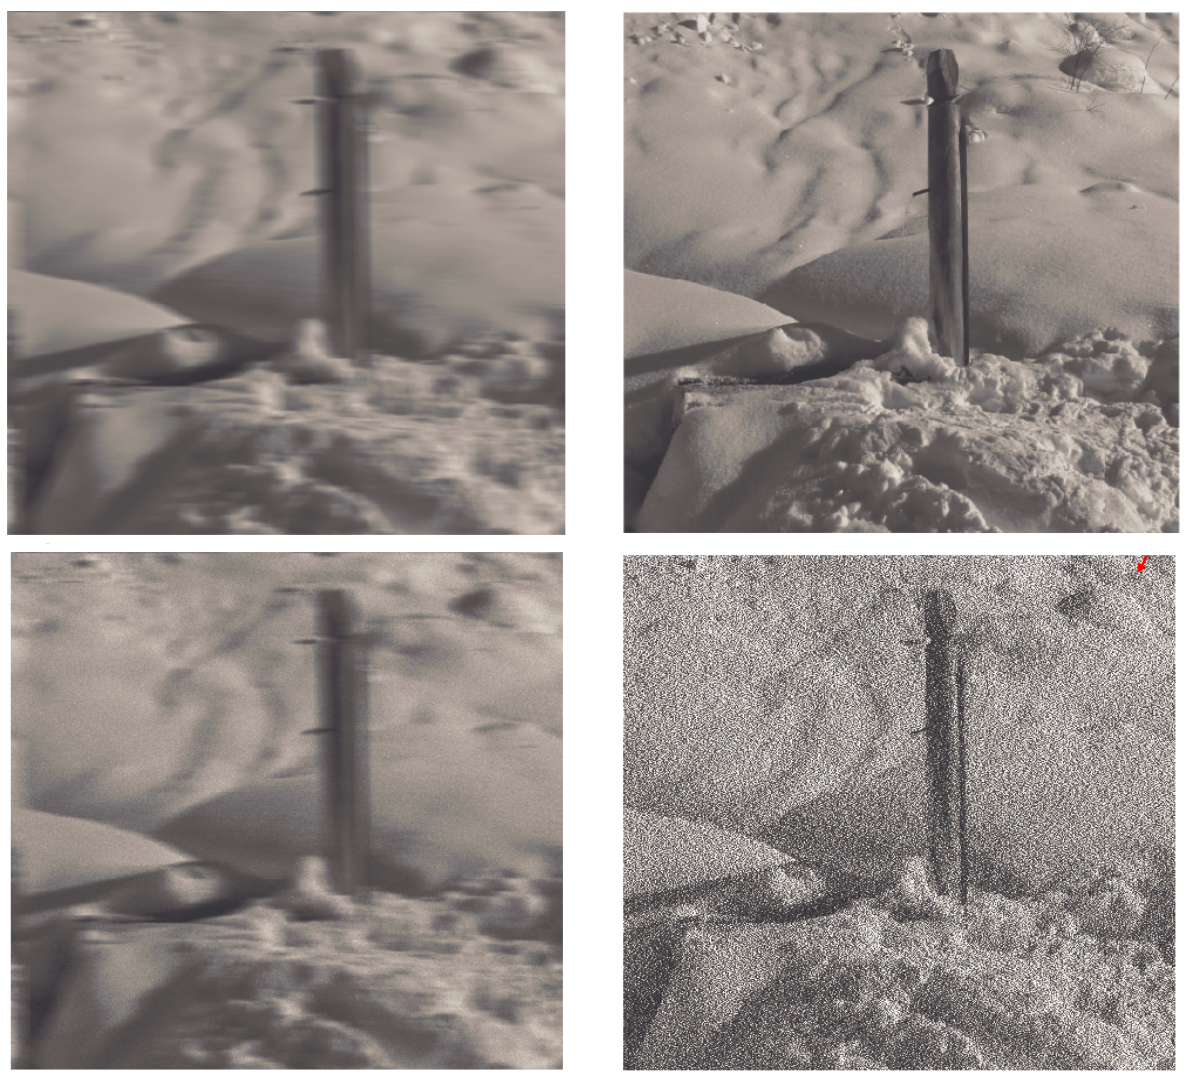
\includegraphics[width=.95\linewidth]{Picture/Inverse_Filter}
\end{wrapfigure}
Dove la frazione indica la deconvoluzione tra il rumore e il filtro che abbiamo usato per ripristinare l'immagine. Dei valori prossimi a zero nel filtro possono aumentare molto la componente rumorosa e l'immagine che si ottiene risulta essere fortemente rovinata, nella figura si vede un esempio di immagine ricostruita con il filtro inverso che è stato modellato seguendo il movimento della camera. La prima coppia di immagini non è affetta da rumore, mentre la seconda sì e anche se nell'immagine mossa il rumore si nota poco in quella ricostruita predomina sull'immagine.

\subsection{Wiener filter}
Il problema del filtro inverso è stato studiatissimo e sono state proposte molte soluzioni che riducessero gli effetti mostrati sopra. Il filtro di Wiener migliora le prestazioni del filtro inverso minimizzando lo scarto quadratico medio (MSE Mean Square Error). Vogliamo minimizzare
\begin{equation}
	E\Big\{(f-\hat{f})^2\Big\}
\end{equation}
Se assumiamo oltre al filtro lineare spazio invariante che il rumore sia decorrelato dall'immagine e che almeno uno tra immagine e rumore abbia media nulla si può ricavare che il minimo del MSE è dato da un'immagine ricostruita con questa forma:
\begin{equation}
	\hat{F}(u,v) = \Bigg[\frac{H^*(u,v)}{|H(u,v)|^2 + S_{\eta}(u,v) / S_f(u,v)}\Bigg]G(u,v)
\end{equation}
Dove:
\begin{itemize}
	\item $H(u,v)$: filtro che ha danneggiato l'immagine
	\item $H^*(u,v)$: complesso coniugato di $H(u,v)$
	\item $|H(u,v)|^2 = H^*(u,v) H(u,v)$
	\item $S_{\eta}(u,v) = |N(u,v)|^2$: spettro di potenza del rumore
	\item $S_f(u,v) = |F(u,v)|^2$: spettro di potenza dell'immagine originale
\end{itemize}
\newpage
Al denominatore vediamo l'inverso del rapporto segnale rumore, infatti $S_{\eta}(u,v) / S_f(u,v) = 1/SNR$. Questo ci dice che il filtro di Wiener diventa il filtro inverso se a una data frequenza il rapporto segnale rumore tende a infinito, mentre cancella le frequenze dominate dal rumore.

È possibile semplificare questo filtro assumendo che il rumore sia bianco, quindi $S_{\eta}(u,v) / S_f(u,v) \rightarrow \sigma^2/ S_f(u,v)$, inoltre dato che in generale lo spettro dell'immagine originale non è noto assumiamo che il rapporto segnale rumore sia costante e lo consideriamo un parametro $K$ del filtro. Il filtro di Wiener diventa quindi:
\begin{equation}
	H(u,v) = \frac{H^*(u,v)}{|H(u,v)|^2 +K} = \frac{1}{H(u,v)}\frac{|H(u,v)|^2}{|H(u,v)|^2 +K} 
\end{equation}

\subsection{CLSF}
Il filtro di Wiener necessita dello spettro dell'immagine e del rumore, o almeno di una loro stima, dato che queste informazioni non sempre sono disponibili sono stati sviluppati altri filtri, come il Constrained Least Squares Filter. Questo filtro parte dall'idea che il filtro inverso fallisce perché il rumore che ha solitamente spettro piatto viene aumentato moltissimo specie alle alte frequenze dove il filtro ha valori molto bassi (ricordiamo che il filtro si trova a denominatore). Per impedire questo effetto si cerca un risultato più smooth minimizzando il laplaciano:

\begin{equation}
	\sum_{x=0}^{M}\sum_{y=0}^{N} \big[\nabla^2f(x,y)\big]
\end{equation}
La soluzione che minimizza il laplaciano è:
\begin{equation}
	\hat{F}(u,v) = \Bigg[\frac{H^*(u,v)}{|H(u,v)|^2 + \gamma|P(u,v)|^2}\Bigg]G(u,v)
\end{equation}
Dove:
\begin{itemize}
	\item $P(u,v)$ è la trasformata dell'operatore laplaciano: $P(u,v) = \mathfrak{F} \Big( \Big[
	\begin{smallmatrix}
		0&-1&0\\
		-1&4&-1\\
		0&-1&0
	\end{smallmatrix} \Big]\Big)$ 
	\item $\gamma$ è un parametro da settare per fare in modo che il filtro riesca effettivamente a isolare il rumore. Siccome $\gamma$ è proprio il parametro più delicato da stimare questo può essere ottenuto \textbf{iterativamente}.
\end{itemize}

\subsection{Filtro con media geometrica}
È possibile generalizzare il filtro di Wiener in uno che ricordi la media geometrica. Questo filtro è molto utile dato che controllando i suoi 2 parametri si possono implementare filtri molto diversi utili in tanti ambiti. Il filtro generale genera un'immagine ricostruita in questo modo:
\begin{equation}
	\hat{F}(u,v) = \left[\frac{H^*(u,v)}{|H(u,v)|^2}\right]^{\alpha}\left[\frac{H^*(u,v)}{|H(u,v)|^2 +\beta\left[\frac{S_{\eta}(u,v)}{S_f(u,v)}\right]}\right]^{1-\alpha}G(u,v)
\end{equation}
Dove $\alpha \geq 0$ e $\beta \geq 0$ sono i parametri e a seconda del loro valore si hanno diversi comportamenti:
\begin{itemize}
	\item $\alpha = 1$: filtro inverso;
	\item $\alpha = 0$: filtro di Wiener parametrico ($\beta$ = 1 Wiener standard);
	\item $\alpha = \frac{1}{2}$: si calcola la media geometrica delle quantità tra parentesi
	\item $\alpha = \frac{1}{2}$ e $\beta = 1$: filtro equalizzatore dello spettro;
	\item $\alpha<\frac{1}{2}$: il filtro si comporta più come Wiener;
	\item $\alpha>\frac{1}{2}$: il filtro si comporta più come filtro inverso.
\end{itemize}
\subsection{Esempi}
\begin{wrapfigure}{r}{.5\linewidth}
	\vspace{-.8cm}
	\centering
	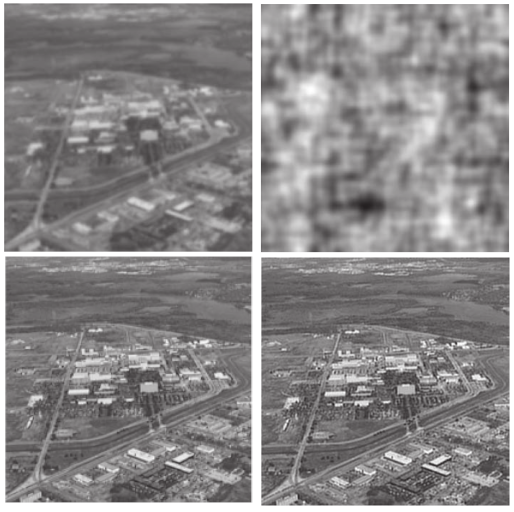
\includegraphics[width=.95\linewidth]{Picture/Filter_Example}
\end{wrapfigure}
Le immagini sono disposte $\left(
\begin{smallmatrix}
	1&2\\
	3&4 
\end{smallmatrix}
\right)
$ e mostrano l'applicazione di diversi filtri a un'immagine rovinata da turbolenza atmosferica e affetta da rumore additivo:
\begin{enumerate}
	\item Immagine originale;
	\item Filtro inverso;
	\item Filtro Wiener;
	\item Filtro CLSF.
\end{enumerate}

\chapter{Low Level Vision}
La low level vision si basa su algoritmi che ricalcano proprietà matematiche per estrarre informazioni utili dalle immagini. Questa branca della computer vision raramente fa uso di intelligenza artificiale e si adatta bene a contesti semplici e controllati come la visione industriale.

La low level vision ha come obbiettivo quello di estrarre delle regioni di interessa dalle immagini, evidenziare bordi e punti di interesse di un'immagine.

\section{Segmentation}
Vogliamo suddividere l'immagine in aree di interesse, cioè creare una maschera che ritagli delle aree dell'immagine semanticamente differenti. La maschera più semplice a cui possiamo pensare ha solo 2 livelli e permette di ottenere un'immagine binarizzata in cui distinguiamo la ragione di interesse dallo sfondo.

\subsection{Thresholding}
È uno dei metodi più intuitivi per fare segmentazione di un'immagine, è molto utilizzato date le se buone proprietà e la pochissima complessità computazionale. Il thresholding permette di dividere i pixel in regioni basandosi sulle proprietà dei pixel stessi.

La forma più semplice di thresholding consiste nel decidere una soglia $T$ e dividere i pixel con intensità minore di $T$ da quelli con intensità maggiore; questo approccio è detto \textbf{thresholding globale}. Se la soglia cambia parliamo invece di thresholding variabile, questo si divide in \textbf{thresholding locale} se $T$ dipende dalle caratteristicche del vicinato del pixel in esame, oppure \textbf{thresholding adattativo} se $T$ dipende dalla posizione nell'immagine.

Lo scopo del thresholding è quello di risolvere un problema decisionale statistico. Vogliamo minimizzare il numero di pixel etichettati nel modo sbagliato.  

Questo significa conoscere la distribuzione dei pixel che rappresentano lo sfondo e la distribuzione dei pixel che rappresentano il soggetto. Stimare le PDF è un problema tutt'altro che semplice, e anche se assumiamo siano distribuzioni normali trovare la soglia ccorretta non è semplice.

\subsubsection{Thresholding globale semplice}
Questo metodo è adatto quando le distribuzioni di pixel sono chiaramente bimodali e la separazione è relativamente facile. La soglia $T$ viene trovata iterativamente raffinando delle stime. L'algoritmo seguito per trovare $T$ è il seguente:
\vspace{.5cm}

\begin{algorithmic}
	\Function{BasicThresholding}{ }
		\State $\Delta T \gets \infty$
		\State $T \gets T_{init}$
		\While{$\Delta T < \Delta T_{min}$}
			\State $G_1 \gets$ \Call{PixelLess}{$T$}
			\State $G_2 \gets$ \Call{PixelGreather}{$T$}
			\State $m_1 \gets$ \Call{IntensityMean}{$G_1$}
			\State $m_2 \gets$ \Call{IntensityMean}{$G_1$}
			\State $T_{new} \gets \frac{m_1 + m_2}{2}$
			\State $\Delta T \gets |T - T_{new}|$
			\State $T \gets T_{new}$
		\EndWhile
	\EndFunction    
\end{algorithmic}

\subsubsection{Thresholding di Otsu}
Al posto di minimizzare i pixel etichettati in modo sbagliato ci concentriamo sul massimizzare la differenza tra le due classi di pixel che separiamo. Questo consiste nel massimizzare la varianza inter-classe (tra le classi).

Il metodo di Otsu è vantaggioso anche perché permette di lavorare unicamente con l'istogramma, che è facile da ottenere e permette di costruire un algoritmo molto efficiente dal punto di vista computazionale.

Avendo $L$ livelli di intensità, un immagine di dimensione $N\times M$ e chiamando $n_i$ il numero di pixel aventi intensità $i$ possiamo la probabilità che un pixel dell'immagine abbia intensità $i$ cioè $p_i = n_i/MN$.

Se scegliamo una soglia $k$ possiamo ora derivare la probabilità che un certo pixel appartenga alla prima ($c_1$) o alla seconda ($c_2$) classe:
\begin{align}
	P_1(k) & = \sum_{i = 0}^{k} p_i\\
	P_2(k) & = \sum_{i = k+1}^{L-1} p_i = 1-P_1
\end{align}
Possiamo calcolare l'intensità media dei pixel in $c_1$, in $c_2$ e la media cumulativa fino al livello $k$ come:
\begin{align}
	m_1(k) & = \sum_{i = 0}^{k} iP(i/c_1) = \frac{1}{P_1} \sum_{i = 0}^{k}ip_i\\
	m_2(k) & = \sum_{i = k+1}^{L-1} iP(i/c_2) = \frac{1}{P_2} \sum_{i = k+1}^{L-1}ip_i\\
	m(k) & = \sum_{i = 0}^{k} ip_i
\end{align}
Definiamo ora la varianza inter-classe come  :
\begin{align}
	\sigma^2_G & = P_1(m_1 - m_G)^2 + P_2(m_2 - m_G)^2= \notag \\
	& = P_1 P_2(m_1-m_2)= \notag \\
	& = \frac{(m_gP_1 - m)^2}{P_1 P_2}
\end{align}
Possiamo ricavare il valore ottimo per la soglia $k^*$ che permette di massimizzare la varianza
\begin{equation}
	\sigma^2_B(k^*) = \underset{0\leq k \leq L-1}{\max} \sigma^2_B(k) = \underset{0\leq k \leq L-1}{\max} \left( \frac{\left[m_gP_1(k) - m(k)\right]^2}{P_1(k)P_2(k)}\right)
\end{equation}

\subsubsection{Migliorare il thresholding globale}
Per migliorare il thresholding globale possiamo usare diverse tecniche:
\begin{enumerate}
	\item moothing dell'immagine;
	\item usare i bordi per individuare la soglia corretta.
\end{enumerate}
\newpage
La prima tecnica consiste nell'applicare un filtro passa basso, facendo \textbf{blurring dell'immagine} possiamo:
\begin{itemize}
	\item ridurre il rumore;
	\item scegliere la dimensione dei dettagli da evidenziare;
	\item passare da un istogramma confuso a uno bimodale.
\end{itemize}

La seconda tecnica si basa sul fatto che tipicamente siamo interessati a separare il soggetto dallo sfondo, se il soggetto ha dei bordi sufficientemente marcati possiamo evidenziarli (ad esempio con il laplaciano) e trovare la soglia di threshold ottima solo sui pixel di bordo. Per fare questo costruiamo una maschera a partire dal laplaciano e la usiamo per selezionare i bordi dell'immagine di partenza. Uno volta trovata la soglia ottima possiamo applicarla a tutta l'immagine.

\subsubsection{Threshold variabile}
\begin{wrapfigure}[20]{r}{.35\linewidth}
	\vspace{-.8cm}
	\centering
	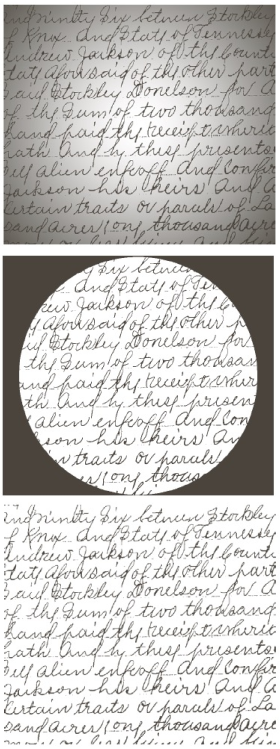
\includegraphics[width=.95\linewidth]{Picture/Moving_Average_Threshold}
\end{wrapfigure}
Compensa un'illuminazione non uniforme definendo per ogni pixel una soglia attraverso strumenti statistici.

Esempi di definizione di soglia sono:
\begin{align*}
	T_{xy} &= a\sigma{xy} +bm_{xy}\\
	T_{xy} &= a\sigma{xy}+bm
\end{align*}

Un esempio più complicato di statistica per scegliere la soglia è quello della \textbf{media mobile}; questa consiste nello scandire l'immagine per riga e risulta particolarmente utile per il riconoscimento del testo. Definiamo la media al passo $k+1$ come
\begin{align}
	m(k+1) &= \frac{1}{n}\sum_{i=k+2-n}^{k+1} z_i =\\ \notag
	               &=m(k)\frac{z_{k+i} - z_{k-n}}{n}
\end{align}
Dove $z_i$ è l'intensità del pixel $i$ e $m(1) = z_1 / n$
Nella figura vediamo l'immagine originale, quella binarizzata col metodo di Otsu e infine qella con la media mobile.

\subsection{Region growing}
Costruiamo le regioni di interesse a partire da un punto che sicuramente vi appartiene (\textbf{seed}) e facciamo crescere la regione aggiungendo pixel che soddisfano una determinata proprietà $Q$.

La parte più complessa di questa procedure è quella di individuare i seed, per fare questo può essere necessario esaminare tutti i pixel dell'immagine per cercare candidati adatti.

Una volta individuati i seed l'algoritmo di region growing è relativamente semplice: per ogni seed individuato si invoca la seguente funzione ricorsiva:
\vspace{.2cm}
\begin{algorithmic}
	\Function{RegionGrowing}{$seed$}
		\State $neighbors \gets $ \Call{8-Connected}{$seed$}
		\ForAll{$pixel$ \textbf{in} $neighbors$}
			\If{\Call{Satisfy}{$Q$,$pixel$}}
				\State $pixel.valid \gets \text{true}$
				\State \Call{RegionGrowing}{$pixel$} 
			\EndIf
		\EndFor
	\EndFunction    
\end{algorithmic}
\vspace{.2cm}
Al termine di ogni chiamata si ottiene una nuova regione di pixel marcati come validi, a questa regione si può poi dare un'etichetta per costruire una maschera.

\subsection{Region splitting and merging}
Questa procedura permette di dividere l'immagine in regioni ricorsivamente più piccole e di raggruppare le regioni adiacenti che rispettano una data proprietà $Q$. La struttura che descrive l'immagine al termine della procedura è un \textbf{quad-tree}; il quad-tree è una struttura molto compatta di rappresentare l'informazione e consente di decidere a priori la grana con cui ricostruire le regini di interesse.

La procedure si divide un due parti, la prima si occupa di dividere le regioni $R$ in sotto-regioni, la seconda di unire le sotto-regioni se entrambe rispettano una proprietà.
\vspace{.1cm}
\begin{algorithmic}
	\Function{Split}{$R$}
		\If{(\textbf{not }\Call{Satisfy}{$Q$,$R$}) \textbf{and} ($R > R_{min}$)}
			\State $R_1$, $R_2$, $R_3$, $R_4$ $\gets \Call{Divide}{R}$
			\State \Call{Split}{$R_1$}, \Call{Split}{$R_2$}, \Call{Split}{$R_3$}, \Call{Split}{$R_4$}
		\EndIf
	\EndFunction    
\end{algorithmic}
\newpage

\begin{algorithmic}
	\Function{Merge}{$region\_set\ R$}
	\DoWhile
		\State $old\_R \gets R$
		\ForAll{$R_a \in R$}
			\ForAll{$R_b \in \Call{Adjacent}{R_a}$}
				\If{\Call{Satisfay}{$Q$,$R_a\cup R_b$}}
					\State$R_{ab} = R_a\cup R_b$
					\State $R  \gets R/\{R_a, R_b\} \cup R_{ab}$
				\EndIf
			\EndFor
		\EndFor
	\EndDoWhile{$R \neq old\_R$}
	\EndFunction    
\end{algorithmic}

\section{Feature Extraction}
Lo scopo della feature extraction è quello di estrarre caratteristiche utili da un'immagine. Non esiste una definizione precisa  e condivisa di cosa sia una feature; in generale le caratteristiche che cerchiamo dipendono dall'appliccazione e dall'elaborazione che seguirà l'estrazione.

A prescindere da cosa consideriamo feature il processo di estrazione si divide un due fasi principali:
\begin{enumerate}
	\item feature detection;
	\item feature description.
\end{enumerate}
Vogliamo cioè non solo individuare le caratteristiche utili, ma essere in grado di descriverle per trovare similitudini e differenze tra feature estratte da diversi punti dell'immagine o tra immagini diverse.

\subsection{Edge Detection}
Sviluppiamo dei metodi per identificare i bordi che siano più robusti e affidabili della semplice derivata (gradiente o laplaciano).

\subsubsection{Marr-Hildreth edge detector}
Questo metodo è molto semplice, non assicura risultati ottimi ma permette di migliorare le prestazioni del detector rispetto al semplice laplaciano. L'idea è che il rumore presente in un immagine può generare falsi positivi, possiamo rimuovere parte di questo disturbo con un filtro gaussiano passa basso. Il filtro ha anche lo scopo di selezionare la dimensione minima dei bordi che vogliamo tenere in considerazione. La procedura per estrarre i bordi è la seguente:
\begin{enumerate}
	\item filtrare l'immagine con un filtro gaussiano passa basso $n\times n$ ($G(x,y)$);
	\item applicare l'operatore laplaciano ($\nabla^2$) al risultato;
	\item trovare i punti di zero crossing.
\end{enumerate}
Possiamo scrivere l'immagine ottenuta al passo 2 come 
\begin{equation}
	g(x,y) = \nabla^2\left[G(x,y)*f(x,y)\right]
\end{equation}
Il punto chiave di questa procedura è quello considerare bordi solo i pixel che si trovano a metà tra due pixel con segno opposto (zero crossing), questo unito al fatto di poter scegliere una soglia minima per il modulo della differenza dei pixel di segno opposto permette di ottenere buoni risultati etichettando bordi fini e precisi.

\subsubsection{Canny edge detector}
È l'algoritmo per l'estrazione dei bordi più complesso, ma che da risultati migliori. Questo metodo ha 3 obbiettivi:
\begin{itemize}
	\item \textbf{basso tasso d'errore}: tutti i bordi devono essere identificati;
	\item \textbf{bordi ben localizzati}: la distanza tra il punto etichettato come bordo e il bordo reale deve essere la minima possibile
	\item \textbf{single point response}: per ogni punto del bordo deve essere etichettato un solo punto, cioè non si devono etichettare i massimi locali nelle prossimità di un  bordo.
\end{itemize}

L'algoritmo è diviso in 4 fasi principali:
\begin{enumerate}
	\item Smoothing dell'immagine con un filtro gaussiano;
	\item Calcolo del gradiente con angolo e modulo;
	\item applicazione della Non Maxima Suppression al modulo del gradiente;
	\item Doppia soglia di theshold per rilevare e unire i bordi.
\end{enumerate}

\textbf{Passo 1}: lo smoothing dell'immagine serve a scegliere la dimensione dei dettagli che ci interessano e permette di rimuovere il rumore che potrebbe portare a falsi positivi.

\textbf{Passo 2}: Calcoliamo il gradiente di ciasun pixel, questo passaggio può essere fatto ad esempio con l'operatore di Sobel che ci fornisce la componente verticale e orizzontale del gradiente, da questa siamo poi in grado di risalire a modulo e direzione.

\begin{wrapfigure}[11]{r}{.35\linewidth}
	\vspace{-.3cm}
	\centering
	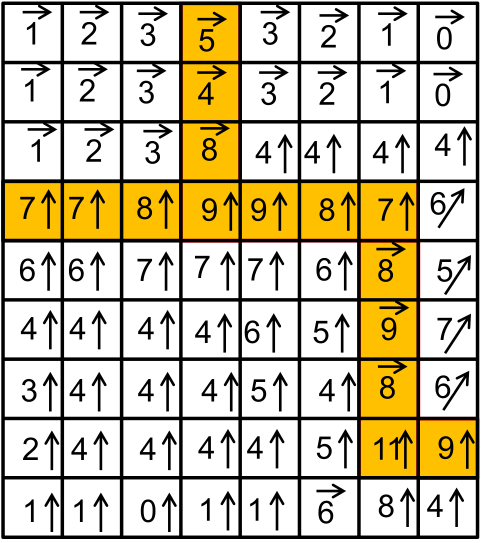
\includegraphics[width=.95\linewidth]{Picture/Canny}
\end{wrapfigure}
\textbf{Passo 3}: Costruiamo una prima approssimazione dei bordi, chiamiamo questa immagine $g_N(x,y)$ e inizializziamo tutti i suoi pixel a 0. Consideriamo i bordi come paralleli a 4 direzioni (verticali, orizzontali e le 2 diagonali), non ci interessa il verso ma solo la direzione. Dato il vettore gradiente del pixel $(x,y)$ in $f$ chiamiamo $d_k$ la direzione (tra le 4 definite prima) più prossima all'angolo del gradiente e $K = ||\nabla f_s||$ il modulo del gradiente. Se $K$ è minore di almeno uno fra i $||\nabla f_s||$
dei picel adiacenti a $(x,y)$ lungo la direzione $d_k$ allora $g(x,y) = 0$ altrimenti $g_N(x,y) = K$.

In questo modo individuiamo un solo punto per ogni bordo, man mano che il gradiente aumenta avvicinandosi al bordo stesso.

\textbf{Passo 4 hysteresis thresholding}: Consideriamo 2 soglie $T_H$ e $T_L$ in rapporto variabile (solitamente tra $2:1$ e  $3:1$) e costriuamo 2 imagini bordi forti $g_{NH}$ e  bordi deboli $g_{NL}$ utilizzando rispettivamente prima e seconda soglia.

In $g_{NH}$, avendo usato una soglia più alta, ci saranno meno pixel. Aggiorno $g_{NL}$ in modo che contenga solo i pixel che mancano a $g_{NH}$ in questo modo: $g_{NL}=g_{NL}-g_{NH}$. I Pixel in $g_{NH}$ vengono marcati tutti come validi, poi per riempire i buchi di questa maschera procedo come segue: 
\begin{enumerate}
	\item etichetto tutti i pixel di $g_{NH}$ come non visitati;
	\item per ogni pixel $(x,y)$ etichettato come non visitato:
	\begin{enumerate}
		\item etichetto come bordo valido tutti i pixel in $g_{NL}$ adiacenti a $(x,y)$;
		\item etichetto $(x,y)$ come visitato;
	\end{enumerate}
\end{enumerate}
Alla fine della procedura tutti i pixel etichettati come validi saranno considerati bordi.

\subsection{Line Detection}

\chapter{AI per la visione artificiale}
\begin{wrapfigure}[7]{r}{.45\linewidth}
	\vspace{-.5cm}
	\centering
	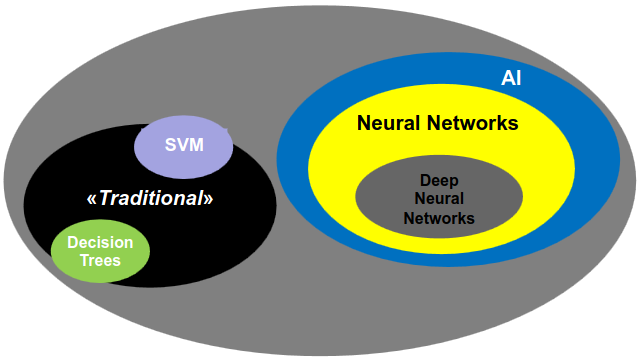
\includegraphics[width=.9\linewidth]{Picture/AI_Classes}
\end{wrapfigure}
L'intelligenza artificiale oggi viene usata in moltissime applicazioni di computer vision e processing di immagini; Le architetture si basano su reti neurali convoluzionali (CNN). In questa trattazione vedremo come si sono evolute le reti neurali partendo dall'idea di percettrone fino ad arrivare alle reti profonde. Per quanto riguarda il metodo di apprendimento ci concentreremo in particolare sull'apprendimento supervisionato.

\section{Percettrone}
Il percettrone è il precursore della moderna AI e cerca di risolvere dei problemi di \textbf{classificazione binaria}. Un problema di questo tipo prevede di riuscire ad etichettare correttamente istanze appartenenti a due classi differenti (esempio: è un cane o un gatto)

\subsection{Funzionamento}
\begin{wrapfigure}[6]{l}{.7\linewidth}
	\vspace{-.2cm}
	\centering
	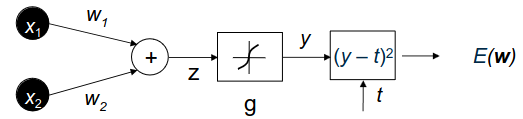
\includegraphics[width=.9\linewidth]{Picture/Perceptron}
\end{wrapfigure}
Nello schema si vede il funzionamento del percettrone, questo calcola una funzione che ha come variabili gli input che riceve e come parametri i pesi $w_i$ degli input. La funzione calcolata è la combinazione lineare degli input pesati e questa serve come input per una funzione di attivazione non lineare, ma differenziabile (tipicamente una \textbf{sigmoide}).
\subsubsection{Aggiornamento dei pesi}\label{sec:stocastic_gradient_descent}
Una volta che è stata calcolata la risposta del percettrone si può calcolare l'errore commesso come scarto quadratico ($E(\vec{w}) = (y - t)^2$) dove $t$ è la classe reale dell'oggetto e può valere 0 o 1. Si può quindi derivare l'errore rispetto al singolo peso con la chain-rule:
\begin{equation}
	\frac{\partial E(\vec{w})}{\partial w_i} = \frac{\partial E}{\partial y} \cdot\frac{\partial y}{\partial z}\cdot \frac{\partial z}{\partial w_i}
\end{equation}
Quindi possiamo aggiornare i pesi considerando il gradiente della funzione errore. Questo metodo si chiama \textbf{stocastic gradient descent}. Passando dall'iterazione $k$ alla $k+1$ possiamo scrivere:
\begin{equation}
	\vec{w}^{k+1} = \vec{w}^k - \eta \nabla_{\vec{w}} E(\vec{w})
\end{equation}
Dove il parametro $\eta$ è detto \textbf{learning rate}, è sempre minore di 1 e influisce su quanto l'errore pesa sull'aggiornamento dei parametri del percettrone.

\subsubsection{Training}
Si inizializzano i pesi casualmente, si calcola l'output per un dato input e si valuta l'errore. Si aggiornano i pesi e si procede in questo modo fino a quando non si esauriscono tutti gli esempi nella classe di training. L'algoritmo
\begin{itemize}
	\item converge se le classi sono linearmente separabili
	\item da come risultato un output binario
\end{itemize}

\section{Multilayer networks}
\begin{wrapfigure}{r}{.45\linewidth}
	\vspace{-.8cm}
	\centering
	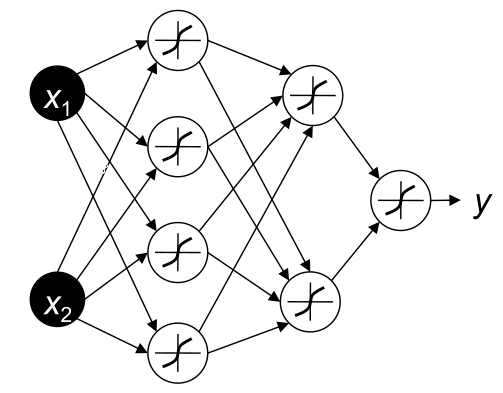
\includegraphics[width=.9\linewidth]{Picture/FCNs}
\end{wrapfigure}
Il singolo neurone permette di classificare classi linearmente separabili. Per poter aumentare la generalità del classificatore si passa alle FCNs (Multilayer Fully Connetted Networks). In queste reti sono presenti uno o più livelli nascosti (hidden), non ci sono cicli e vi è un layer di output.
\newpage
\subsection{Funzionamento}
\begin{wrapfigure}[13]{l}{.63\linewidth}
	\vspace{-.1cm}
	\centering
	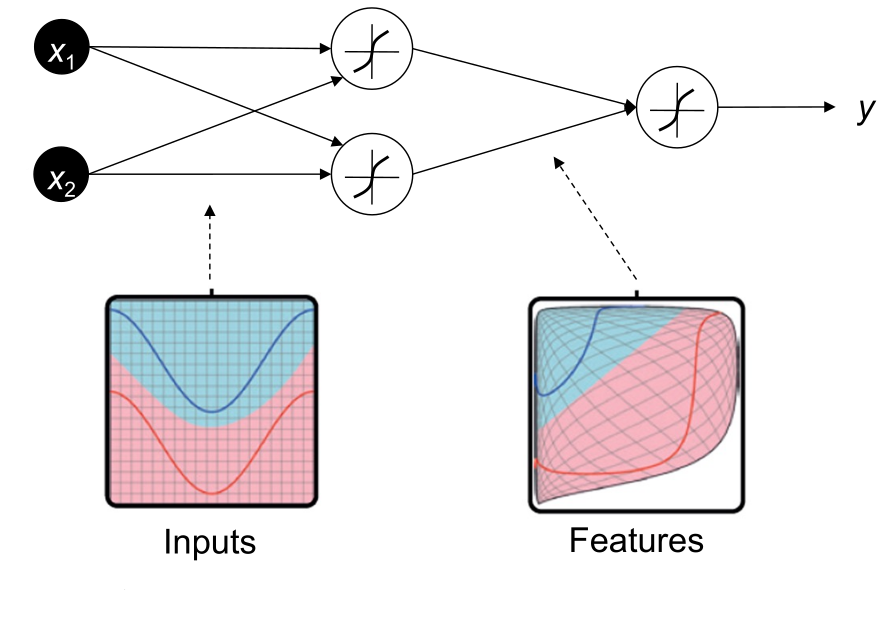
\includegraphics[width=.95\linewidth]{Picture/FCNs_Mapping}
\end{wrapfigure}
I livelli hidden hanno lo scopo di rendere le features linearmente separabili in modo che il livello di output possa operare come descritto prima per il percettrone. L'operazione dei livelli nascosti è quindi una trasformazione dallo spazio degli input allo \textbf{spazio latente} dove si spera che la classificazione sia più semplice. 

Più sono i livelli hidden più è complessa la funzione che si può apprendere per separare le classi.
\subsubsection{Complessità}
La complessità è data dal numero di parametri che devono essere appresi. Per ogni livello il numero di pesi sarà il prodotto tra il numero di input di ogni neurone (+ 1 per il bias)  e il numero di neuroni del layer ovvero il numero di output del layer stesso. Formalmente:
\begin{equation}
	N_{par} = n_{out} \cdot (1+n_in)
\end{equation}

\subsection{Overfitting}
Man mano che si aggiungono livelli e si aumenta la complessità della rete i le funzioni che possono essere apprese diventano sempre più complesse, questo può portare al fenomeno dell'\textbf{overfitting}; che si verifica quando la rete apprende troppo bene i parametri per minimizzare l'errore sul set di training e perde quindi di generalità. Questo fenomeno è evidenziato da un grosso divario tra i punteggi realizzati sul set di training e sul set di validation.

\newpage
\subsubsection{Esempio}
Consideriamo di dover interpolare dei punti con una curva, l'immagine mostra come al variare del numero di gradi di libertà abbiamo 
\begin{multicols}{3}
	\begin{itemize}
		\item underfitting
		\item good fitting
		\item overfitting
	\end{itemize}
\end{multicols}
\begin{center}
	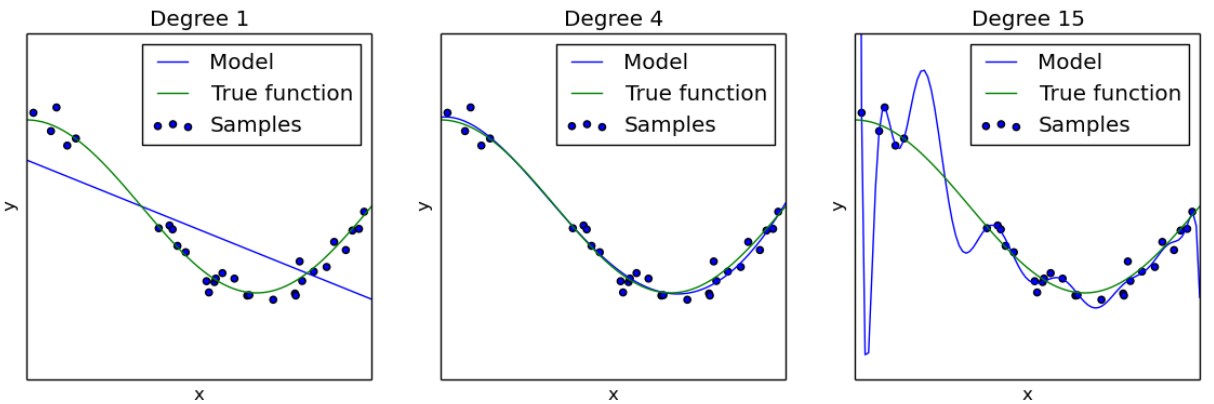
\includegraphics[width=\linewidth]{Picture/Overfitting}
\end{center}
Nell'ultimo caso stiamo fittando il rumore e non i dati.
\subsubsection{Regularization}\label{sec:regularization}
Per impedire l'overfitting si ricorre alla regolarizzazione. Dall'esempio si può immaginare che per far fluttuare così rapidamente la funzione che fa overfitting è necessario che i suoi coefficienti abbiano un \say{grande} valore assoluto. Si cerca di penalizzare le soluzioni con pesi elevati, minimizzando 
\begin{equation}
	J(\vec{w})= E(\vec{w}) + \lambda R(\vec{w}) = E(\vec{w}) + \lambda ||\vec{w}|| ^2
\end{equation}
Dove $R(\vec{w})$ è un fattore di normalizzazione che solitamente si traduce nella norma al quadrato le vettore dei pesi e $\lambda$ è un parametro che normalmente è qualche ordine di grandezza più piccolo del learning rate $\eta$.

\subsection{Multiclass Classification}
Quando abbiamo più di due classi usiamo un livello di output che contiene tanti neuroni quante sono le classi da riconoscere, in questo modo quando incontriamo un oggetto appartenente a una classe si attiva solo il neurone corrispondente e gli altri dovrebbero rimanere spenti. Nella pratica però è raro che si attivi un solo neurone al $100\%$ e gli altri rimangano spenti. Nei casi fortunati avremo un neurone molto attivo e gli altri poco, non è detto però che la somma degli output dei vari neuroni sommi a 1.
\newpage
\subsubsection{Livello Soft-Max}
\begin{wrapfigure}[8]{r}{.6\linewidth}
	\vspace{-.8cm}
	\centering
	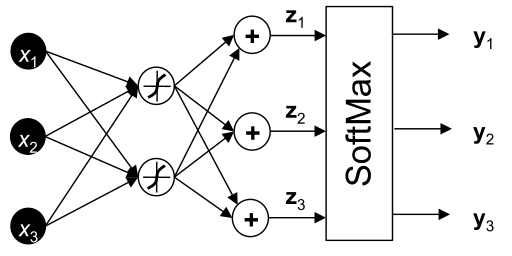
\includegraphics[width=.95\linewidth]{Picture/Multiclass_Soft_Max}
\end{wrapfigure}
Se la somma delle attivazioni dei neuroni non è 1 non possiamo trattarla come una distribuzione di probabilità (PDF). Per risolvere questo problema si aggiunge un livello di normalizzazione che scala gli output dei neuroni e ci assicura di poter trattare il risultato come una PDF.  Per trasformare il risultato dei neuroni in una PDF si usa la formula:
\begin{equation}
	y_i= \sigma(\vec{z})_i = \frac{e^{z_i}}{\sum_{k = 1}^{n} e^{z_k}}  \qquad\text{con } i = 1, 2, \dots, n 
\end{equation}



\subsection{Loss function}
Fino ad ora abbiamo calcolato la funzione d'errore come scarto quadratico (MSE).  Questa politica però ha dei problemi, dato che nella funzione del calcolo dell'errore rientrano anche gli errori dovuti alle classi sbagliate che tendono a spingere $\vec{y}$ verso 0; questo può portare a una distribuzione meno mirata dell'errore.
Definiamo allora la \textbf{Cross Entropy Loss Function} come
\begin{equation}
	L(y, t) = - \sum_i t_i \log(y_i) = - \log(y_{i*})
\end{equation}
Dove $y_{i*}$ è la risposta del neurone associato alla classe corretta e si ottiene dalla sommatoria dato che tutti gli altri $t_i$ valgono 0.

Il risultato di usare la Cross Entropy è:
\begin{itemize}
	\item  l'errore e quindi il gradiente propagato attraverso la rete deriva solo dalla classe corretta $i*$ e ne consegue un aggiornamento dei pesi può mirato;
	\item  all'inizio del training i gradienti sono più grandi e questo porta alla convergenza più rapida dei pesi.
\end{itemize}

\section{Riconoscere immagini}
Ora che abbiamo costruito un sistema in grado di apprendere proviamo a insegnargli a riconoscere le immagini. Il primo tentativo in tal senso è stato fatto per riconoscere le cifre da 0 a 9.

\subsection{LeNet 300}\label{sec:LeNet300}
Il primo compito di classificazione delle immagini consisteva nel riconoscimento di cifre. Queste erano salvate come immagini $28\times28$, in scala di grigi con profondità di 8 bit e contenute in un dataset chiamato \textbf{MNIST}
\subsubsection{Architettura}
\begin{wrapfigure}[6]{r}{.45\linewidth}
	\vspace{-1cm}
	\centering
	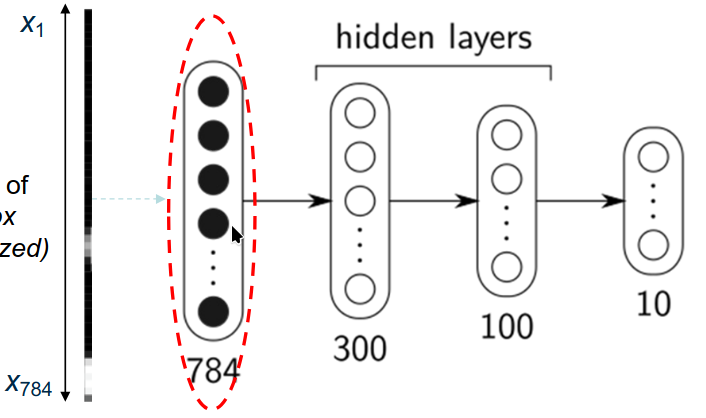
\includegraphics[width=.9\linewidth]{Picture/LeNet_300}
\end{wrapfigure}
La LeNet 300 è una FCN prevede un livello di input costituito da $784$ neuroni, uno per ogni pixel dell'immagine. Ci sono poi 2 livelli hidden costituiti da 300 e 100 neuroni rispettivamente, infine un livello di output costituito da 10 neuroni. La funzione di attivazione del livello di input e dei livelli hidden è una sigmoide, mentre per il livello di output si usa una Soft-Max.
\subsubsection{Pro e contro}
La LeNet migliora le sue performance man mano che si aggiungono livelli hidden e raggiunge, nella configurazione presentata, un tasso di errore del $3.05\%$. 

Aggiungere altri livelli però produrrebbe un grosso incremento della complessità e richiederebbe set di immagini molto grandi per evitare overfitting. Inoltre una FCN non si adatta bene allo scalare delle dimensioni dell'immagine, infatti per ogni pixel è necessario un neurone sul layer di input, questo significa moltissimi neuroni appena si utilizzano immagini di risoluzione maggiore.

\subsection{Un approccio diverso}
Le FCNs prevedono una serializzazione dell'immagine, ogni pixel è mandato a un neurone. Questo però non è come un immagine dovrebbe essere trattata. Le immagini infatti sono caratterizzate da elevata correlazione spaziale, se si serializzano si conserva la correlazione in una sola dimensione.

I filtri, d'altro canto, si comportano così bene sulle immagini perché mantengono la correlazione tra i dati.

Viene quindi naturale pensare di poter applicare l'apprendimento automatico alla costruzione di filtri per riuscire a estrarre le features che più ci interessano per raggiungere il nostro scopo. I pesi dei filtri saranno proprio i parametri che la rete deve apprendere al fine di estrarre le features importanti. Nascono in questo modo le \textbf{reti convoluzionali}.
\chapter{Convolutional Neural Network}

\section{Neurone convoluzionale}
\begin{wrapfigure}{l}{.6\linewidth}
	\vspace{-.2cm}
	\centering
	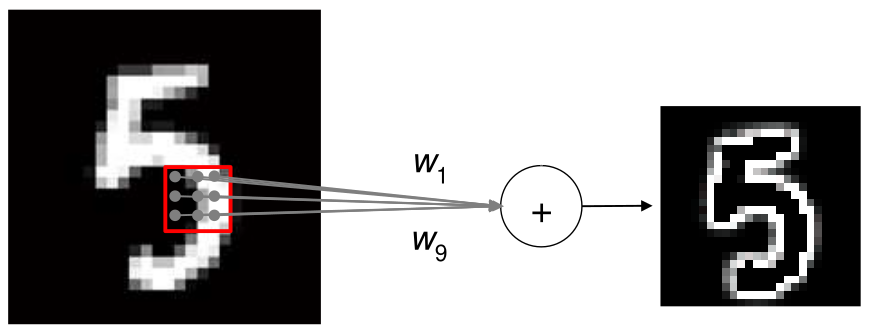
\includegraphics[width=.9\linewidth]{Picture/Convolutional_Neuron}
\end{wrapfigure}
È un neurone che applica un filtro all'immagine ed estrae la tessa feature da tutta l'immagine. Per fare questo opera come un normale neurone che calcola una combinazione lineare degli input, ma gli input avranno dei vincoli spaziali, in particolare saranno una matrice quadrata di pixel che con la convoluzione viene filtrata dai parametri del neurone. I parametri saranno appressi attraverso la backpropagation e non si dovranno più progettare a mano i filtri per estrarre le features.

Per fare in modo che dopo l'operazione di filtraggio il risultato abbia le stesse dimensioni dell'immagine originale si fa zero padding. 

Se stiamo trattando immagini colorate trattiamo ogni canale in modo indipendente, ad esempio se costruiamo dei filtri $3\times3$ ogni neurone apprenderà $27$ parametri, $9$ per ogni filtro. I risultati del filtraggio dei tre canali è poi sommato per generare la feature map.

\section{Complessità del layer convoluzionale}
Il numero di parametri che devono essere appresi per ogni livello convoluzionale sarà dato dal numero di feature map che vlgiamo ottenere $n_{out}$ (numero di filtri nel livello) per la dimensione del filtro + 1 per il numero di canali in ingresso; questi saranno 3 per le immagini a colori 1 per e immagini in scala di grigi e  il numero di feature map estratte al livello precedente se stiamo considerando un generico layer all'interno della rete.  In formule possiamo scrivere:
\begin{equation}
	N_{par} = n_{out} \cdot (1+F^2)\cdot n_{ch}
\end{equation}
Dove $F$ rappresenta il lato del filtro.
\subsection{Complessità della rete}
Ogni neurone convoluzionale restituisce come output un'immagine delle stesse dimensioni dell'immagine originale. Dopo che abbiamo estratto tutte le feature che ci interessano quindi dobbiamo tornare a una FCN per poter fare la classificazione. Per fare questo semplicemente serializziamo ogni feature map e la concateniamo con le altre.

Il collo di bottiglia diventa quindi il layer di passaggio tra CNN e FCN, dato che al posto di avere un neurone per ogni pixel dell'immagine originale avremo un neurone per ogni pixel di ogni feature map, e queste possono essere anche molte.

\subsection{Ridurre la complessità}
Per ridurre la complessità possiamo trattare le feature map come immagini e sottocampionarle. Per ridurre le dimensioni delle feature map abbiamo due alternative.

\subsubsection{MaxPolling}
\begin{wrapfigure}{r}{.5\linewidth}
	\vspace{-.5cm}
	\centering
	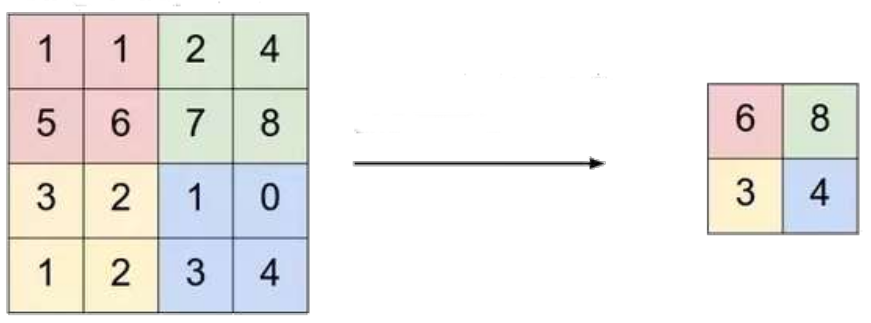
\includegraphics[width=.9\linewidth]{Picture/MaxPolling}
\end{wrapfigure}
Il MaxPolling consiste nel dividere l'immagine in celle da 4 pixel e per ogni cella prendere solo il valore maggiore. In questo modo dimezziamo la dimensione dell'immagine e dato che prendiamo solo il valore più grande e non facciamo la media eseguiamo anche un'operazione di \textbf{Non Maxima Suppression}, si è visto che questo aggiunge robustezza alle traslazioni.

\subsubsection{Convolve and Stride}
In questo caso ogni convoluzione ha un passo maggiore di 1, questo significa che il flitro non si sposta sull'immagine pixel per pixel ma fa dei salti.

Questa tecnica non prevede la Non Maxima Suppression, ma è parte integrante del processo di filtraggio e non deve essere aggiunta come layer intermedio tra 2 layer di neuroni. Questo rende la tecnica del convolve and stride più flessibile e di fatto ha soppiantato il MaxPolling nelle moderne architetture.

\section{LeNet5}
Presentiamo l'architettura della LeNet5 che prevede 2 livelli convoluzionali da 6 e 16 neuroni, intervallati da 2 livelli di MaxPolling, si passa poi 3 livelli FC. 
\begin{center}
	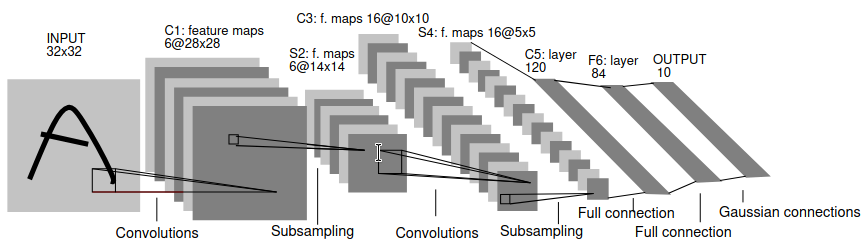
\includegraphics[width=.8\linewidth]{Picture/LeNet_5}
\end{center}
Il tasso d'errore della LeNet5 con l'architettura in figura è di $0.95\%$, questo miglioramento nelle performance è accompagnato anche da una riduzione della complessità della rete rispetto alla LeNet300, in particolare il numero di parametri necessari alla LeNet5 è meno di $\frac{1}{3}$ dei parametri necessari alla LeNet300.

\section{Receptive Field}
Il receptive field di una feature indica quanti pixel dell'immagine originale sono stati usati per generare la feature. Ad esempio un filtro $3\times3$ ha un receptive field di 9 pixel.

Nell'immagine si vede una rappresentazione 2D del receptive fiel della LeNet5. Notiamo che:

\begin{wrapfigure}[4]{r}{.5\linewidth}
	\vspace{-.5cm}
	\centering
	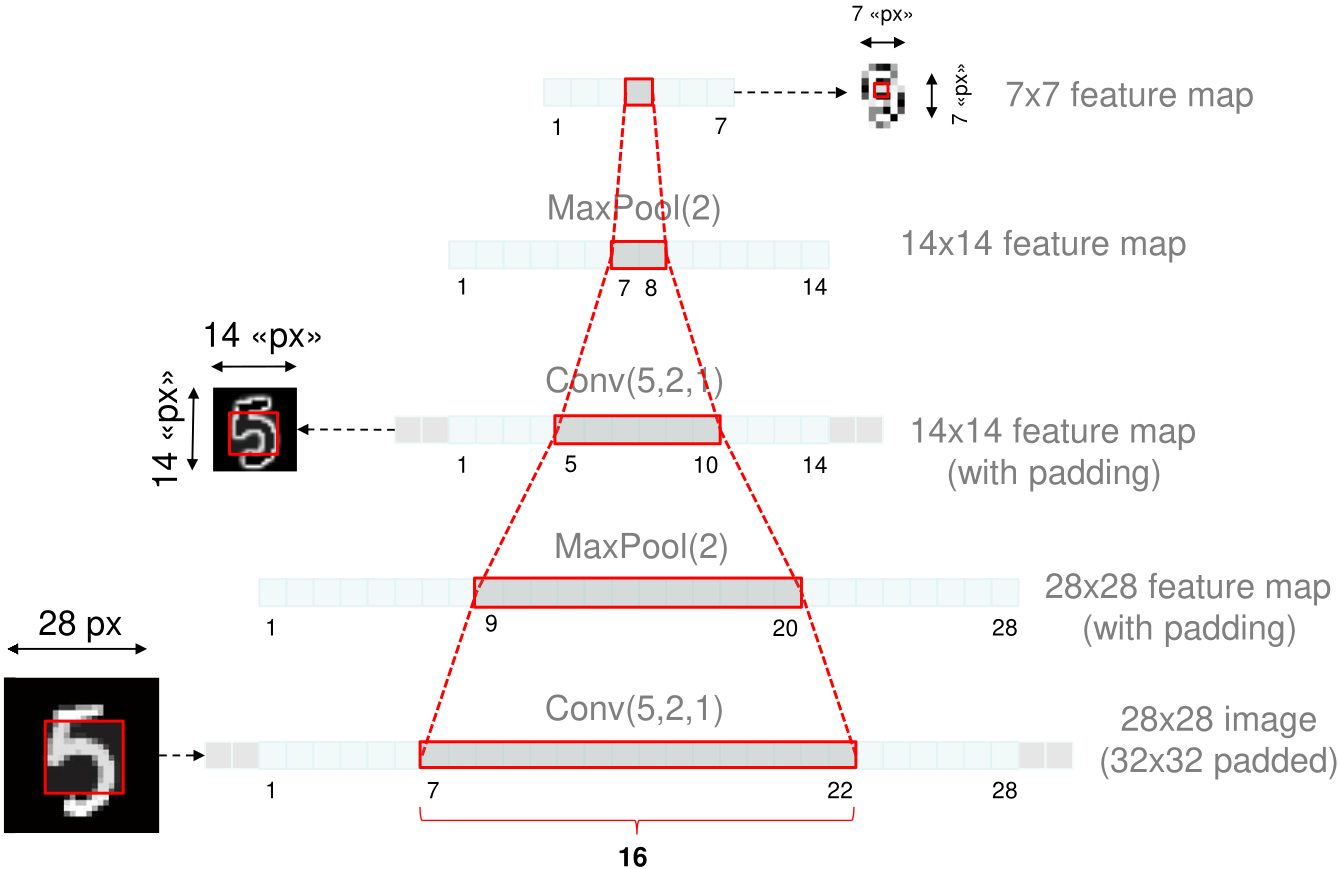
\includegraphics[width=\linewidth]{Picture/Receptive_Field}
\end{wrapfigure}
\ 
\vspace{-.5cm}
\begin{itemize}
	\item i livelli di MaxPolling sono quelli che più di tutti influiscono sul receptive fiel, raddoppiandolo;
	\item i filtri aumentano la dimensione del receptive field per effetto del padding.
\end{itemize}

	Che si usi il MaxPolling oppure il convolve and stride il subsampling dell'immagine consente di aumentare il receptive field. Questo è molto importante perché vogliamo che ogni feature (che al passando dall'ultimo livello convoluzionale al primo fully connected è costituita da un pixel) trasporti più informazione possibile.
	
\section{Da fully connetted a fully convolutional}
\subsection{Riconosimento del testo}
Ora che abbiamo progettato una rete in grado di raggiungere elevata acccuratezza nel riconoscimento dei singoli caratteri vorremmo poter leggere il testo scritto su in immagine. Per fare questo abbiamo bisogno di individuare i caratteri prima di riconoscerli. L'approccio naif consiste nel:
\begin{itemize}
	\item aggiungere una classe di backgound che non corrisponde a nessun carattere;
	\item aggiungere una classe che corrisponde all'intersezione di 2 caratteri, anche questa non corrisponde a nessun carattere;
	\item fare zigzag per l'immagine con passo di 1 pixel per individuare tutti i caratteri.
\end{itemize}
Questo approccio è molto inefficiente, dato che ogni pixel viene elaborato molte volte, tutte le elaborazioni sono indipendenti e la maggior parte di queste sono ridondanti o non portano informazione.
\subsection{Sliding Window}
Al posto che ritagliare l'immagine in quadrati della stessa dimensione delle immagini di training posso usare delle finestre di dimensione arbitraria, tanto i livelli convoluzionali si comportano come filtri e possono essere applicati a qualsiasi immagine.

\begin{wrapfigure}{l}{.53\linewidth}
	\vspace{-.25cm}
	\centering
	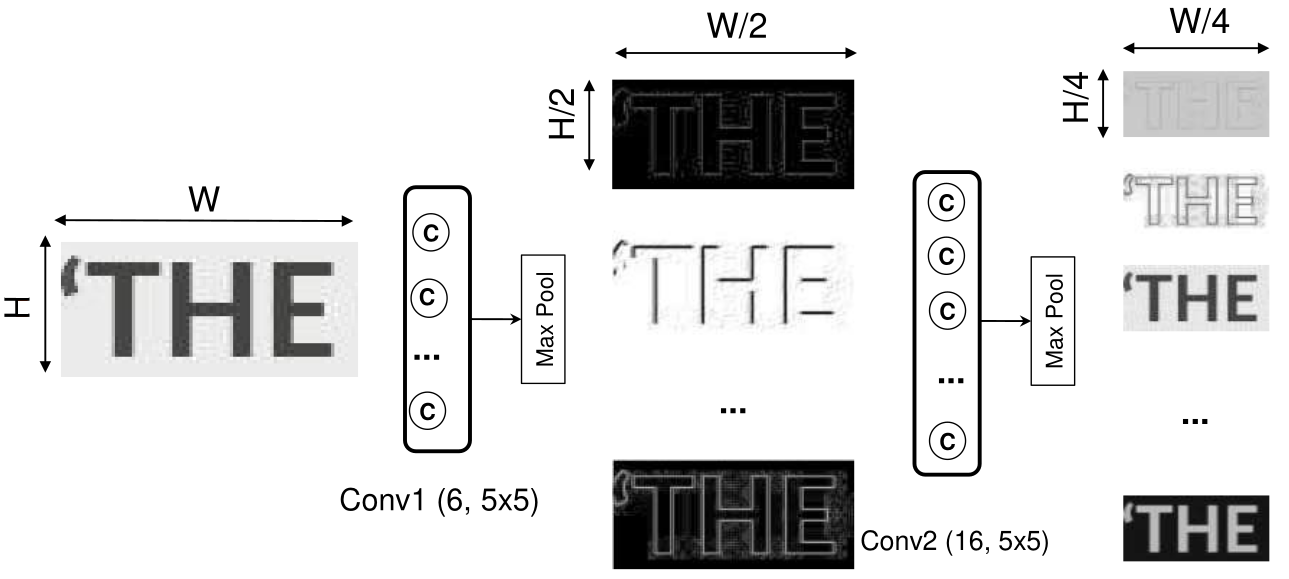
\includegraphics[width=\linewidth]{Picture/Sliding_Window_LeNet_5}
\end{wrapfigure}
Nella figura si vede l'effetto dei neuroni convoluzionali che permettono di estrarre le feature per le quali sono stati addestrati da un immagine qualsiasi. Si vede anche l'effetto del MaxPolling che dopo ogni livello dimezza la dimensione delle features. 

Rimane però un problema, dato che la rete termina con dei livelli fully connected questi hanno bisogno di un vettore di input di dimensione fissata e non possono adattarsi alle dimensioni della finestra arbitraria che abbiamo scelto.

\subsection{Equivalente convoluzionale}
\begin{wrapfigure}{r}{.5\linewidth}
	\vspace{-.25cm}
	\centering
	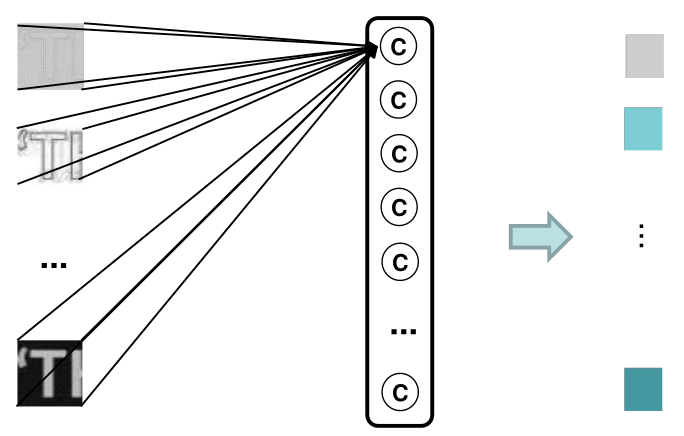
\includegraphics[width=\linewidth]{Picture/FC_To_CNN}
\end{wrapfigure}
Sostituiamo quindi i livelli fully connected con dei livelli convoluzionali. Consideriamo il primo livello FC, questo riceve in input un certo numero di features map (FM) di dimensione fissa. Per ogni FM avrà un peso per ogni pixel. Possiamo quindi trasformare questo neurone in un filtro semplicemente trattandolo come tale senza bisogno di cambiare i pesi. I neuroni convoluzionali ottenuti trasformando un layer FC sono detti \textbf{narrow}. Anche il livello di output può essere sostituito con un livello convoluzionale collegato poi alla funzione Soft-Max.

Una volta fatte queste sostituzioni siamo pronti per applicare la rete fully convolutional (CNN) all'intera immagine
\begin{center}
	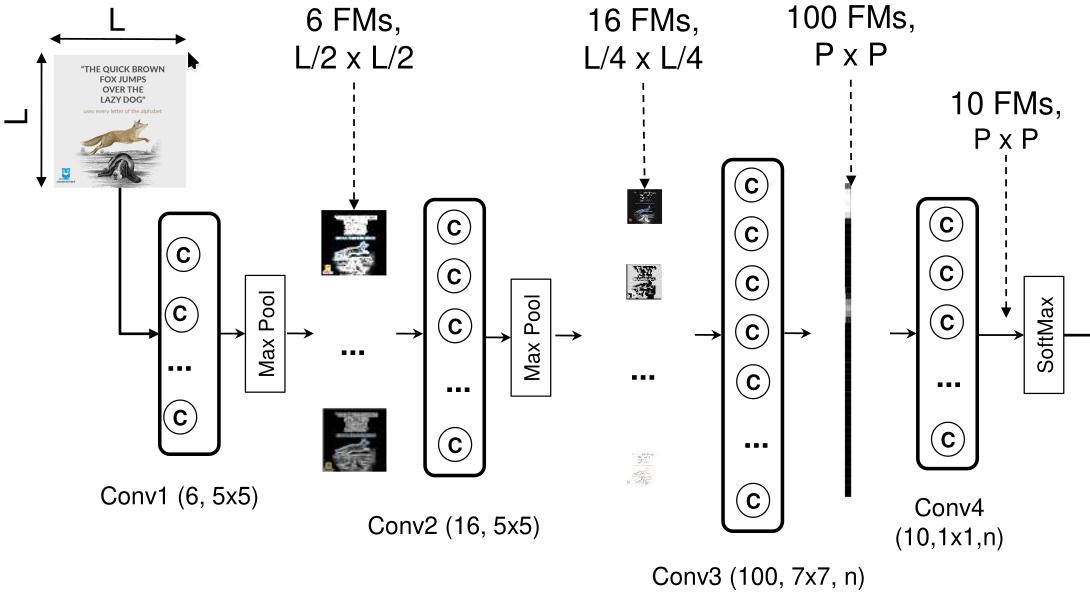
\includegraphics[width=.75\linewidth]{Picture/CNN}
\end{center}
Dove:
\begin{equation}
	P = 1 + \frac{L -(f_{dim} \cdot 2^{n_{pools}})}{4}
\end{equation}
e $f_{dim}$ è la dimensione del filtro narrow del primo livello FC tradotto (in questo caso la dimensione è 7), e $n_{pools}$ è lo stride (In questa rete quindi si combinano convolve and stride e MaxPolling).
\subsection{Interpretare i risultati}
{\Huge DA RISCRIVERE}

\begin{wrapfigure}{r}{.4\linewidth}
	\vspace{-.25cm}
	\centering
	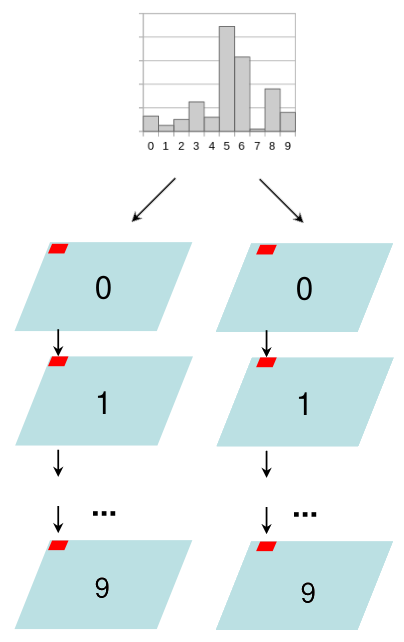
\includegraphics[width=\linewidth]{Picture/Post_CNN}
\end{wrapfigure}
Ora che abbiamo ottenuto delle feature map dobbiamo interpretarle. Per fare questo possiamo riutilizzare il classificatore FC che avevamo prima convertito in convoluzionale e passare a questo dei vettori di lunghezza 10, ciascun vettore conterrà il pixel $i,j$ di ciascuna delle 10 FM che abbiamo estratto con la rete CNN. Ogni vettore può quindi essere classificato e fornirci in output un carattere. Nel caso della LeNet5 si ottengono 10 FM $19\times19$, saremo quindi in grado di riconoscere al massimo $19\times19 = 361$ caratteri.

 Il risultato di questa prima interpretazione potrebbe essere ancora poco soddisfacente, potrebbero infatti esserci dei doppioni e delle lettere sbagliate. A valle di questo passaggio quindi si usano dei language model e altre reti per raffinare il risultato da un punto di vista semantico. 
 
\chapter{Advanced Learning}
Nei capitoli precedenti (\ref{sec:stocastic_gradient_descent}) abbiamo visto come minimizzare una certa funzione di loss usando il gradiente
\begin{equation}
	\vec{w}^{k+1} = \vec{w}^k - \eta \nabla_{\vec{w}} E(\vec{w})
\end{equation}
Ci domandiamo ora come rendere efficiente il training, sia modificando i parametri dell'equazione appena mostrata sia modificando proprio la strategia di learning.

\section{Learning rate}
La scelta del learning rate corretto è fondamentale per avere una rete che converga al minimo globale dell'errore, infatti se abbiamo learning rate
\begin{multicols}{3}
	\begin{itemize}
		\item troppo piccolo finiremo incastrati in minimi locali;
		\item corretto riusciamo a individuare il minimo globale;
		\item troppo grande la rete non converge a un minimo.
	\end{itemize}
\end{multicols}
\begin{center}
	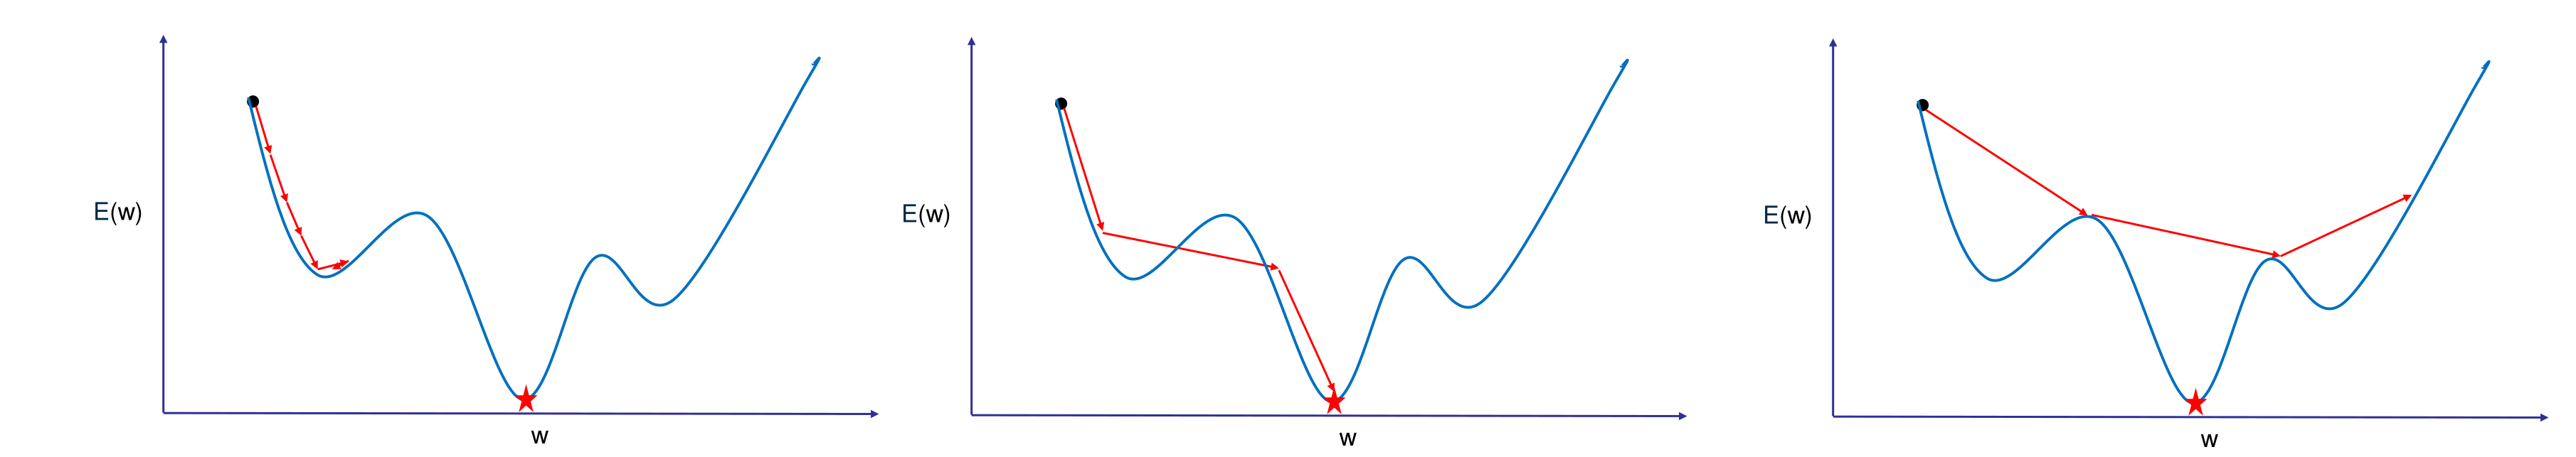
\includegraphics[width=\linewidth]{Picture/Learning_Rate}
\end{center}

L'idea è che all'inizio dell'allenamento la rete si strovi a grande distanza dal minimo globale, man mano che vengono appresi i pesi ci si avvicina e gli step verso il minimo si fanno più piccoli. Per sfruttare questa idea si può modificare il learning rate durante l'apprendimento.

\subsection{Decadimento del learning rate}
Per modificare il learning rate possiamo seguire diverse politiche, in questo paragrafo ci concentriamo sulle più semplici che sono monotone decrescenti, ma esistono alti modi di far variare il learnin rate che non sono monotoni e possono riuscire a non incastrarsi in minimi locali.
\subsubsection{Step decay}
Dopo in certo numero di iterazioni (\textbf{epoche}) il learning rate viene moltiplicato per un valore $<1$ in modo da rendere il suo grafico un decadimento esponenziale a gradini. Le epoche in cui avviene la riduzione del learning rate sono dette \textbf{milestones}. Formalmente a ogni milestones il learning rate viene aggiornato in questo modo:
\begin{equation}
	\eta = \eta_0 \cdot e^{-kt}
\end{equation}
dove $\eta_0$ è il learning rate iniziale, $k$ è il numero della milestones e $t$ è un parametro.
\subsubsection{Time decay}
Dopo ogni epoca il learning rate iniziale viene diviso per  il numero di epoche opportunamente pesato. In questo caso il grafico del learning rate è un ramo di iperbole. Formalmente
\begin{equation}
	\eta = \frac{\eta_0}{1 + k\cdot t}
\end{equation}
dove $\eta_0$ è il learning rate iniziale, $k$ è il numero dell'epoca attuale e $t$ è un parametro.
\subsubsection{Exponential decay}
Come lo step decay, ma l'aggiornamento viene fatto dopo ogni epoca. Formalmente
\begin{equation}
	\eta = \eta_0 \cdot e^{-kt}
\end{equation}
dove $\eta_0$ è il learning rate iniziale, $k$ è il numero dell'epoca attuale e $t$ è un parametro.
\newpage
\section{Stocastic gradient descent}
\begin{wrapfigure}{r}{.5\linewidth}
	\vspace{-.25cm}
	\centering
	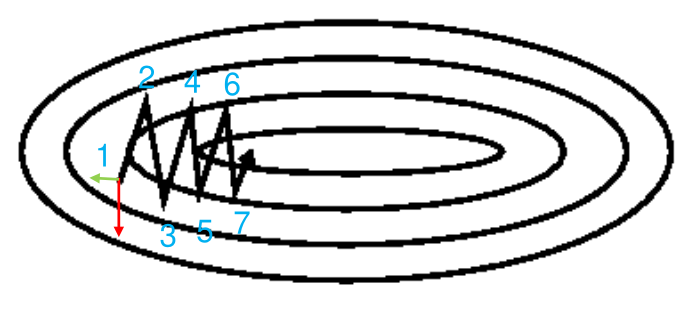
\includegraphics[width=\linewidth]{Picture/SGD}
\end{wrapfigure}
Lo stocastic gradient descent SGD presenta dei problemi quando incontriamo una valle, infatti se osserviamo la situazione dell'immagine è facile convincersi che mentre le frecce verdi rimarranno costanti e orientate verso il minimo le frecce rosse invertono il loro segno ogni volta, questo provoca una discesa a zigzag dell'errore (poco efficiente). Quando si verifica lo zigzag diciamo che il \textbf{gradiente è rumoroso} in quella dimensione, dato che cambia tutte le volte di segno.

\subsection{Aggiunta della quantità di moto}
Per limitare il rumore di alcune componenti del gradiente si può ricorrere a delle similitudini con la fisica. Una pallina lanciata nel punto 1 farà poche oscillazioni ampie, per poi accelerare maggiormente verso il minimo. Esattamente come mostrato nell'immagine.

\begin{wrapfigure}{l}{.5\linewidth}
	\vspace{-.25cm}
	\centering
	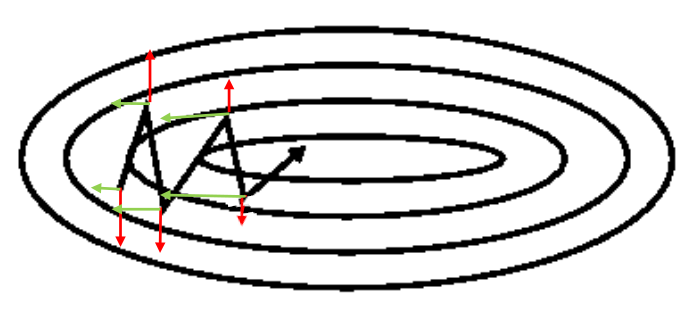
\includegraphics[width=\linewidth]{Picture/SGD_Momentum}
\end{wrapfigure}
Per replicare questo comportamento si aggiunge una sorta di conservazione della quantità di moto (in inglese momentum) che si oppone all'oscillare del segno delle componenti rumorose del gradiente. La componente inerziale che aggiungiamo al gradiente è semplicemente il gradiente calcolato all'iterazione precedente. Formalmente all'iterazione $k+1$ avremo:
\begin{equation}
	\vec{w}^{k+1} = \vec{w}^k - \eta (\nabla_{\vec{w}} E(\vec{w}^k) + \nabla_{\vec{w}} E(\vec{w}^k))
\end{equation}

\subsection{Tecniche avanzate di discesa del gradiente}
Sono stati ingegnerizzati moltissimi altri ottimizzatori ciascuno che punta a risolvere le criticità dei precedenti. La maggior parte di questi è già implementata nei framework per l'AI, Pythorch offre:
\begin{multicols}{4}
	\begin{itemize}
		\item Adadelta
		\item Adagrad
		\item Adam
		\item ASDG
		\item LBFGS
		\item Rprop
		\item SDG
		\item Ecc\dots
	\end{itemize}
\end{multicols}

\section{Batch Training}
In uno scenario ideale tutti i campioni del set di training ci portano verso il minimo globale, nella realtà pero i dati del set possono essere  effetti da errore, questo fa si che campione per campione il minimo si trovi in posizione diversa e questo porta a oscillare intorno al minimo piuttosto che a raggiungerlo.

Per mitigare l'effetto degli errori e del rumore nei campioni di training si ricorre a tecniche statistiche.

\subsection{Minibatch}
Al posto che addestrare la rete campione per campione si divide il set di training in minibatch di $m$ campioni. E si usano i risultati dell'addestramento sull'intero mini batch per aggiornare i pesi della rete.
\vspace{.5cm}
\begin{algorithmic}
	\Function{MiniBatchTraining}{}
		\ForAll {minibatch $b$ in $trainingSet$}
			\State $\vec{G} \gets 0$ \Comment{init. accumulatore gradiente}
			\ForAll{sample $x$ in $b$}
				\State $y \gets$ \Call{NetInference}{x} \Comment{risultato della rete}
				\State $E \gets$ \Call{LossFunction}{y}
				\State $\vec{g} \gets \nabla_{\vec{w}}E(\vec{w})$ \Comment{Calcolo gradiente}
				\State $\vec{G} \gets \vec{G} + \vec{g}$ \Comment{Accumulo gradienti}
			\EndFor
			\State $\vec{w}^{b + 1} \gets \vec{b} + \eta \frac{1}{m} \vec{G}$ \Comment{Aggiorno pesi con la media del gradiente}
		\EndFor
	\EndFunction    
\end{algorithmic}

\begin{wrapfigure}[5]{r}{.3\linewidth}
	\vspace{-1.2cm}
	\centering
	\includegraphics[width=.9\linewidth]{Picture/Batch_Training1}
	\includegraphics[width=.9\linewidth]{Picture/Batch_Training2}
\end{wrapfigure}
\vspace{.5cm}
L'immagine mostra le differenze tra un addestramento sample per sample e uno fatto con i minibatch. Questo approccio
\begin{itemize}
	\item permette convergenza più rapida dovuta ai minori errori
	\item è la chiave delle architetture profonde
	\item rendere computazionalmente efficiente il training
	\item permette di mischiare immagini di classi diverse in un solo aggiornamento dei pesi
\end{itemize}

\section{Overfitting}
Nel capitolo introduttivo (\ref{sec:regularization}) abbiamo già parlato di come la regolarizzazione possa prevenire l'overfitting, vediamo ora altre tecniche che di solito vengono usate in aggiunta alla regolarizzazione.

\subsection{Data Augmentation}
Dato che le reti neurali hanno bisogno di moltissimi esempi per l'addestramento quelli nel set di training possono non essere sufficienti. Si ricorre allora alla data augmentation che consiste nel sintetizzare nuove immagini a partire da quelle presenti nel set.

Per sintetizzare nuove immagini si può ricorrere a diverse trasformazioni, modificando ad esempio:

\begin{wrapfigure}[5]{r}{.6\linewidth}
	\vspace{-.7cm}
	\centering
	\includegraphics[width=.9\linewidth]{Picture/Data_Augmentation}
\end{wrapfigure}
\ 
\vspace{-.5cm}
\begin{multicols}{2}
	\begin{itemize}
		\item Scala
		\item Rotazione
		\item Traslazione
		\item Blur
		\item Contrasto
		\item Luminosità
		\item Proiezione
		\item Ecc\dots
	\end{itemize}
\end{multicols}
\vspace{.5cm}
L'immagine mostra esempi di data augmentation relativi a un set di immagini per il riconoscimento dei frutti. Ovviamente non tutte le trasformazioni sono ammissibili, ad esempio se dobbiamo riconoscere del testo non possiamo ruotare di $180^{\circ}$ i caratteri.

Grazie alla data augmentation possiamo aunentare la diversità intra-classe dei dati, si è visto sperimentalmente che questo approccio porta a vantaggi notevoli, ad esempio la LeNet300 che abbiamo presentato prima (\ref{sec:LeNet300}) dopo la data augmentation passa da un tasso di errore del $3.05\%$ a uno del $2.45\%$

\subsection{Committees of Neural Networks}
L'overfitting è spesso causato dal fatto che ci sono troppi pochi campioni perchè una rete complessa possa apprendere la generalità del problema. Questo approccio quindi consiste nel dividere la rete complessa in tante reti più semplici e unire i risultati degli output di ciascuna per prendere la decisione finale. In questo modo si riduce il numero di parametri di ciascuna rete e si previene l'overfitting. 

È importantissimo in questo caso inizializzare i pesi delle sotto-reti in modo attento, non vogliamo avere tante copie di una rete, ma molte reti diverse ciascuna cche ha appreso in modo diverso come risolvere il problema.

In base alla tipologia del problema si potranno unire i risultati in modo diverso:
\begin{itemize}
	\item \textbf{Classificazione}: il risultato definitivo sarà quello più votato dalle sotto-reti;
	\item \textbf{Regressione}: il risultato può essere ottenuto facendo la media dei risultati forniti.
\end{itemize}

\subsection{Dropout}
Per rendere più snella la rete un fase di training si possono interrompere alcuni collegamenti nei vari layer, i neuroni alimentati da questi collegamenti resteranno spenti. 

\begin{wrapfigure}{r}{.4\linewidth}
	\vspace{-.7cm}
	\centering
	\includegraphics[width=.9\linewidth]{Picture/Dropout1}
	\includegraphics[width=.9\linewidth]{Picture/Dropout2}
\end{wrapfigure}
La strategia tipica è quella di scegliere un certo tasso di dropout e ogni neurone avrà quella porpbabilità di essere disattivato.

I neuroni spenti non partecipano alla creazione dell'output, né al calcolo del gradiente, inoltre i loro pesi non saranno aggiornati.

Terminato il training tutti i neuroni partecipano all'inferenza, ma l'output di ciscun neurone sarà ridotto in proporzione al tasso di dropout, per compensare l'assenza delle attivazioni durante il training.

Nell'immagine si vede un esempio di rete sottoposta a dropout. Questa tecnica funziona perché permette alla rete di distribuire l'apprendimento su tutti i neuroni e non far affidamento solo su alcuni (o su specifiche connessioni tra neuroni), è come se si addestrassero tante sotto-reti tutte diverse ad ogni iterazione; rendendo la rete più robusta a piccole variazioni nel training set e rendendo l'apprendimento più generale
\backmatter
% bibliography, glossary and index would go here.

\end{document}